\documentclass[11pt,a4paper]{article}

% Packages
\usepackage[utf8]{inputenc}
\usepackage[T1]{fontenc}
\usepackage{lmodern}
\usepackage[margin=2.5cm]{geometry}
\usepackage{booktabs}
\usepackage{graphicx}
\usepackage{amsmath}
\usepackage{amssymb}
\usepackage{hyperref}
\usepackage{xcolor}
\usepackage{float}
\usepackage{caption}
\usepackage{longtable}
\usepackage{fancyhdr}

% Page style
\pagestyle{fancy}
\fancyhf{}
\fancyhead[L]{CCM Billet Tracking System --- Comprehensive Analysis}
\fancyhead[R]{\thepage}
\renewcommand{\headrulewidth}{0.4pt}

% Hyperref setup
\hypersetup{
    colorlinks=true,
    linkcolor=blue!60!black,
    citecolor=blue!60!black,
    urlcolor=blue!60!black
}

% Title
\title{\textbf{Comprehensive Analysis} \\ CCM Billet Tracking System Simulation}
\author{Simulation Framework: SimPy 4.1 DES \\ Configuration: Correction Plan v3 (C1--C8, A1--A12)}
\date{2026-02-25}

\begin{document}

\maketitle
\tableofcontents
\newpage

%======================================================================
\section{Introduction and Scope}
\label{sec:introduction}

This report evaluates the CCM (Continuous Casting Machine) billet handling chain capacity after implementing all corrections specified in Correction Plan~v3. The billet handling chain consists of:

\begin{enumerate}
    \item \textbf{Torch cut} --- Oxy-fuel torch severs the billet from the moving strand
    \item \textbf{Transport roller table} --- Carries billets 25.2\,m from torch cut to discharge area
    \item \textbf{Discharge roller table} --- 13.375\,m run with intermediate and fixed stoppers; pairs billets for transfer. The intermediate stopper is located 7.175\,m from the discharge entry. A billet travelling at 15\,m/min reaches it in $7.175 / 15.0 \times 60 = 28.7$\,s. This 28.7\,s transit time is the detection window for traffic jams (see Section~\ref{sec:stopper-timing} for full stopper timing derivation)
    \item \textbf{Transfer car} --- C-hook car lifts billet pairs and travels to cooling bed
    \item \textbf{Cooling bed} --- 84-slot walking beam; billets traverse in 2016\,s
    \item \textbf{Collecting table} --- Pusher groups billets into packs of~2
    \item \textbf{Overhead cranes} --- Two cranes (108 west, 109 east) transport packs to storage yard
    \item \textbf{Billet yard} --- $186 \times 32.45$\,m storage area with stacking up to 20 layers
\end{enumerate}

The simulation uses SimPy~4.1 with a 7200\,s (2-hour) runtime and 1200\,s warmup period. Jam detection and all statistics are computed only after warmup. The primary question addressed is:

\begin{center}
\textbf{What is the maximum safe casting velocity for 6-strand operation?}
\end{center}

%======================================================================
\section{Correction Plan v3 Summary}
\label{sec:correction-plan}

\subsection{Corrections (C1--C8)}

\begin{table}[H]
\centering
\caption{Correction Plan v3 --- Corrections}
\label{tab:corrections}
\begin{tabular}{@{}clllp{5cm}@{}}
\toprule
ID & Parameter & Before & After & Impact \\
\midrule
C1 & Torch travel distance & 3\,750\,mm & 2\,100\,mm & Shorter torch engagement \\
C2 & TC long travel speed & 100\,m/min & 24\,m/min & TC travel times $\sim$4$\times$ longer \\
C3 & TC initial position & Undefined & 4.2\,m from str.~3--4 & Realistic starting point \\
C4 & Stopper configuration & One stopper & Two per strand & Proper pairing sequence \\
C5 & Billet entry point & Torch modeled & Transport RT start & Cleaner model boundary \\
C6 & RT speed & Fixed 15\,m/min & Variable 0--15 & Noted as variable \\
C7 & Crane \& yard params & Guessed & Full yard drawing data & Realistic distances/zones \\
C8 & Crane cycle time & Fixed 350\,s & Parametric formula & Accurate crane timing \\
\bottomrule
\end{tabular}
\end{table}

\subsection{Key Additions}

\begin{table}[H]
\centering
\caption{Correction Plan v3 --- Key Additions}
\label{tab:additions}
\begin{tabular}{@{}clp{8cm}@{}}
\toprule
ID & Addition & Description \\
\midrule
A1 & Strand lag modes & Deterministic (paired 20\,s offsets) and stochastic \\
A6 & Stopper event logging & Security/intermediate hit times in data model \\
A7 & Crane grab rotation & 1\,rev/min, $90^\circ$ rotation = 15\,s \\
A8 & Variable hook drop & $h_\text{drop} = 9.0 - (\text{layer}-1) \times 0.130$\,m \\
A9 & Crane anti-collision & 15\,m min gap, crane 108 always west of 109 \\
\bottomrule
\end{tabular}
\end{table}

\subsection{Aggregate Impact}

The single most consequential correction was \textbf{C2} (TC speed $100 \to 24$\,m/min). Combined with corrected distances:
\begin{itemize}
    \item TC ceiling dropped from 4.21 to \textbf{2.19\,m/min} (theoretical)
    \item Crane cycle dropped from $\sim$350 to \textbf{274\,s} (layer~1, C8 formula)
    \item Torch travel per cut dropped from 3.75 to \textbf{2.1\,m} (C1)
\end{itemize}

%======================================================================
\section{Hand Calculations --- Theoretical Limits}
\label{sec:hand-calcs}

\subsection{Transfer Car Ceiling (Critical Calculation)}

The transfer car serves all 6 strands serially. Each strand produces a pair of billets every $2 \times t_\text{cycle}$ seconds. The TC must collect from all 6 strands within one pair production interval.

\textbf{Strand-to-cooling-bed distances} (at $v_\text{TC} = 24$\,m/min):

\begin{table}[H]
\centering
\caption{TC strand distances and travel times}
\label{tab:tc-distances}
\begin{tabular}{@{}crrr@{}}
\toprule
Strand & Distance (m) & One-Way (s) & Round Trip (s) \\
\midrule
1 & 10.2 & 25.50 & 51.00 \\
2 & 8.9 & 22.25 & 44.50 \\
3 & 7.6 & 19.00 & 38.00 \\
4 & 6.3 & 15.75 & 31.50 \\
5 & 5.0 & 12.50 & 25.00 \\
6 & 3.7 & 9.25 & 18.50 \\
\bottomrule
\end{tabular}
\end{table}

Travel time formula: $t = d / v_\text{TC} \times 60$ (distance in metres, speed in m/min, result in seconds).

\textbf{Average round trip:}
\begin{equation}
\bar{t}_\text{RT} = \frac{51.00 + 44.50 + 38.00 + 31.50 + 25.00 + 18.50}{6} = \frac{208.50}{6} = 34.75\;\text{s}
\end{equation}

\textbf{Hook operations per strand service:}
\begin{equation}
t_\text{hook} = 4 \times 5.0 = 20.0\;\text{s}
\end{equation}

(Hook down at strand, hook up, hook down at cooling bed, hook up.)

\textbf{Average TC cycle per strand:}
\begin{equation}
\bar{t}_\text{TC} = \bar{t}_\text{RT} + t_\text{hook} = 34.75 + 20.0 = 54.75\;\text{s}
\end{equation}

\textbf{Total TC time for all 6 strands:}
\begin{equation}
T_\text{TC,6} = 6 \times 54.75 = 328.5\;\text{s}
\end{equation}

\textbf{Pair production time:}
\begin{equation}
T_\text{pair} = 2 \times \frac{L}{v} \times 60 = \frac{720}{v}\;\text{s}
\end{equation}

\textbf{TC ceiling:}
\begin{equation}
\boxed{v_\text{max,TC} = \frac{720}{328.5} = 2.19\;\text{m/min}}
\end{equation}

Above 2.19\,m/min, the TC cannot serve all 6 strands within one pair production cycle. The deficit accumulates until a billet reaches the security stopper while it is still raised.

\subsection{Billet Timing at Key Velocities}

Billet cycle time $= L/v \times 60$ where $L = 6.0$\,m. Torch travel time $= 2.1/v \times 60$.

\begin{table}[H]
\centering
\caption{Billet timing at key velocities}
\label{tab:billet-timing}
\begin{tabular}{@{}lrrrrl@{}}
\toprule
Parameter & $v{=}1.5$ & $v{=}2.0$ & $v{=}2.3$ & $v{=}3.0$ & Unit \\
\midrule
Billet cycle time & 240.0 & 180.0 & 156.5 & 120.0 & s \\
Torch travel time & 84.0 & 63.0 & 54.8 & 42.0 & s \\
Cast-only time & 156.0 & 117.0 & 101.7 & 78.0 & s \\
Pair production time & 480.0 & 360.0 & 313.0 & 240.0 & s \\
TC margin & $+151.5$ & $+31.5$ & $-15.5$ & $-88.5$ & s \\
TC margin (\%) & 46.1 & 9.6 & $-5.0$ & $-26.9$ & --- \\
\bottomrule
\end{tabular}
\end{table}

At $v = 2.0$\,m/min, the TC has only 31.5\,s of margin (9.6\%) per 6-strand cycle. At $v = 2.3$\,m/min, the margin goes negative by 15.5\,s.

\subsection{Crane Cycle Calculation}

\textbf{Pickup sequence} (constant, at collecting table):
\begin{align}
t_\text{hook\_down} &= 9.0 / 10.0 \times 60 = 54.0\;\text{s} \\
t_\text{grab\_close} &= 5.0\;\text{s} \\
t_\text{hook\_up} &= 54.0\;\text{s} \\
t_\text{pickup} &= 113.0\;\text{s}
\end{align}

\textbf{One-way travel} (130$\times$130 avg distances: 40.0\,m longitudinal, 15.0\,m transverse):
\begin{equation}
t_\text{travel} = \max\!\left(\frac{40.0}{100.0}\times 60,\;\frac{15.0}{40.0}\times 60\right) = \max(24.0,\;22.5) = 24.0\;\text{s}
\end{equation}

\textbf{Placement} (layer~1, no height offset):
\begin{align}
t_\text{hook\_drop} &= (9.0 - 0 \times 0.130) / 10.0 \times 60 = 54.0\;\text{s} \\
t_\text{placement} &= 54.0 + 5.0 + 54.0 = 113.0\;\text{s}
\end{align}

\textbf{Full crane cycle (layer~1):}
\begin{equation}
\boxed{T_\text{crane} = 113.0 + 24.0 + 113.0 + 24.0 = 274.0\;\text{s}}
\end{equation}

\textbf{Crane throughput limit:}
\begin{equation}
v_\text{max,crane} = \frac{1440 \times P}{274 \times N}
\end{equation}
where $P$ = packs per trip, $N$ = number of strands.

\subsection{Stopper Timing --- Hand Calculation}
\label{sec:stopper-timing}

The discharge roller table has three stopper positions. All transit times use the roller table speed of 15\,m/min.

\textbf{Step 1: Positions (measured from transport RT entry)}

\begin{table}[H]
\centering
\caption{Stopper positions and transit times}
\label{tab:stoppers}
\begin{tabular}{@{}lcc@{}}
\toprule
Stopper & Position from Transport RT Entry & Calculation \\
\midrule
Security stopper & 25.2\,m (end of transport RT) & Fixed \\
Intermediate stopper & $25.2 + 7.175 = 32.375$\,m & Security + 7.175\,m into discharge \\
Fixed stopper & $25.2 + 13.375 = 38.575$\,m & Security + full discharge length \\
\bottomrule
\end{tabular}
\end{table}

\textbf{Step 2: Transit times from transport RT entry}
\begin{align}
\text{Security:}\quad & 25.2 / 15.0 \times 60 = 100.8\;\text{s} \\
\text{Intermediate:}\quad & 32.375 / 15.0 \times 60 = 129.5\;\text{s} \\
\text{Fixed:}\quad & 38.575 / 15.0 \times 60 = 154.3\;\text{s}
\end{align}

\textbf{Step 3: Inter-stopper gaps on discharge RT}

The 28.7\,s value is the time for a billet to travel from the discharge entry to the intermediate stopper:
\begin{equation}
t_\text{entry to intermediate} = \frac{7.175}{15.0} \times 60 = 28.7\;\text{s}
\end{equation}

The gap from intermediate to fixed stopper:
\begin{equation}
t_\text{intermediate to fixed} = \frac{13.375 - 7.175}{15.0} \times 60 = \frac{6.200}{15.0} \times 60 = 24.8\;\text{s}
\end{equation}

\textbf{Step 4: Why 28.7\,s matters for traffic jam detection}

When the second billet of a pair enters the discharge RT, it takes 28.7\,s to reach the intermediate stopper. During this 28.7\,s window, even if the TC is slightly behind schedule, no jam occurs because the billet is still in transit. The collision check happens at the security stopper (end of transport RT), not at the discharge entry. A third billet arriving at the raised security stopper while the pair is still waiting for TC pickup triggers a traffic jam.

%======================================================================
\section{Safe Operating Point --- $v = 2.0$\,m/min}
\label{sec:safe-point}

2.0\,m/min is the highest casting velocity that runs jam-free across all tested seeds.

\subsection{Key Performance Indicators}

\begin{table}[H]
\centering
\caption{KPIs at $v = 2.0$\,m/min}
\label{tab:kpi-2.0}
\begin{tabular}{@{}lr@{}}
\toprule
Metric & Value \\
\midrule
Billets produced & 228 \\
Billets delivered to yard & 142 \\
Jam & NO \\
TC utilization & 86.1\% \\
TC average cycle time & 55.7\,s \\
Avg wait for TC & 152.9\,s \\
Max wait for TC & 266.8\,s \\
Avg cooling bed occupancy & 27.4 slots \\
Max cooling bed occupancy & 36 slots \\
Avg collecting table packs & 1.20 \\
Max collecting table packs & 3 \\
Primary bottleneck & Transfer car (86\%) \\
\bottomrule
\end{tabular}
\end{table}

\subsection{Bottleneck Analysis}

\begin{table}[H]
\centering
\caption{Wait times at $v = 2.0$\,m/min}
\label{tab:waits-2.0}
\begin{tabular}{@{}lrr@{}}
\toprule
Wait Point & Avg Wait (s) & Max Wait (s) \\
\midrule
Discharge RT (for TC) & 60.8 & 157.2 \\
Transfer car & 152.9 & 266.8 \\
Collecting table (for crane) & 73.1 & 137.0 \\
\bottomrule
\end{tabular}
\end{table}

The transfer car is the binding constraint at 86.1\% utilization. The crane system operates well below capacity --- collecting table packs never exceed~3 (capacity is~7).

\subsection{TC Margin Validation --- Hand Calculation vs Simulation}

\textbf{How to verify the ``228 billets produced'' number:}
\begin{align}
\text{Billet cycle time at 2.0\,m/min} &= 6.0 / 2.0 \times 60 = 180\;\text{s} \notag\\
\text{Billets per strand over 7200\,s} &= 7200 / 180 = 40 \notag\\
\text{Expected total (6 strands)} &= 6 \times 40 = 240 \notag\\
\text{Actual (simulation)} &= 228 \notag\\
\text{Difference:}\quad & 12\;\text{billets (5\%) due to startup lags (strands 2,3,5,6 start 20--40\,s late)} \notag
\end{align}

\textbf{How to verify the ``86.1\% TC utilization'' number:}
\begin{align}
\text{TC average cycle} &= 55.7\;\text{s per strand (simulation measured)} \notag\\
\text{TC total for 6 strands} &= 6 \times 55.7 = 334.2\;\text{s} \notag\\
\text{TC cycles completed} &\approx 69\;\text{(from simulation log)} \notag\\
\text{TC busy time} &= 69 \times 55.7 = 3843\;\text{s (approximate)} \notag\\
\text{Utilization} &= \text{total logged busy time} / \text{sim end time} = 86.1\% \notag
\end{align}

\textbf{Hand calculation vs simulation:}

\begin{table}[H]
\centering
\caption{TC margin: hand calculation vs simulation at $v = 2.0$\,m/min}
\label{tab:tc-margin-compare}
\begin{tabular}{@{}lrrlp{3.5cm}@{}}
\toprule
Metric & Hand Calc & Simulation & Gap & Reason \\
\midrule
Pair production time & 360.0\,s & --- & --- & Fixed formula \\
TC time for 6 strands & 328.5\,s & 334.2\,s & $+1.7\%$ & Queuing delays \\
TC margin & 31.5\,s (9.6\%) & 25.8\,s (7.2\%) & --- & Sim margin is smaller \\
\bottomrule
\end{tabular}
\end{table}

The $+0.95$\,s per-strand queuing delay arises when the TC arrives at a strand before the pair is fully assembled and waits briefly.

\subsection{Plots --- Safe Operating Point}

\begin{figure}[H]
\centering
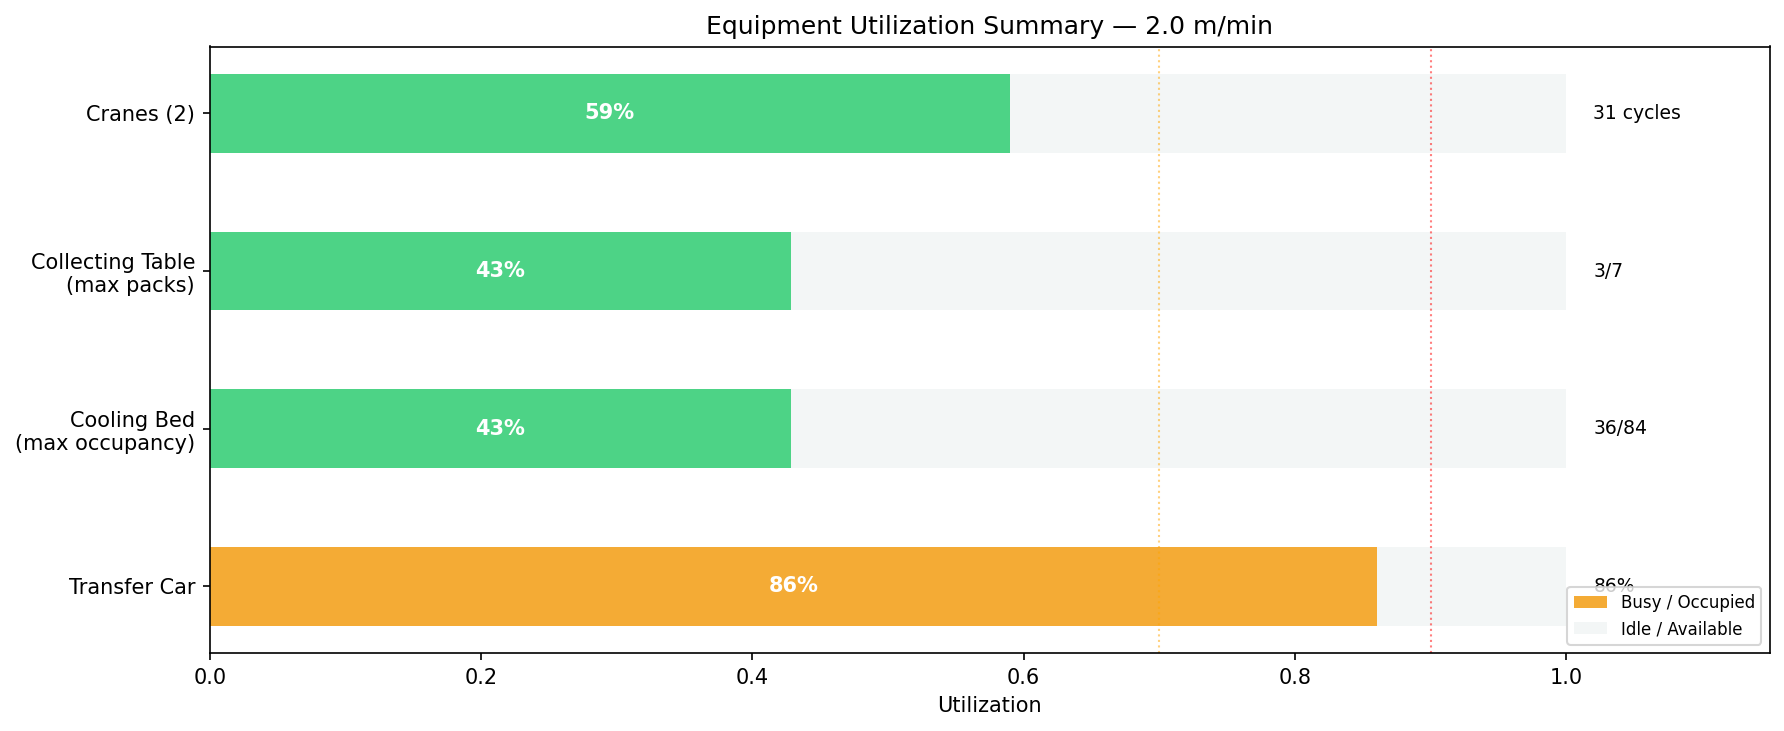
\includegraphics[width=0.85\textwidth]{output/v2.0/V5_equipment_utilization.png}
\caption{Equipment utilization at $v = 2.0$\,m/min. TC is the highest-utilized equipment at 86\%.}
\label{fig:v2.0-util}
\end{figure}

The utilization chart shows four metrics. For the transfer car and cranes, the bar represents \textbf{time-averaged utilization} (fraction of simulation time spent actively working). For the cooling bed and collecting table, the bar represents \textbf{peak capacity fraction} (maximum slots or packs observed divided by total capacity). These are different metrics: the collecting table ``max packs'' bar shows $3/7 = 43\%$ peak capacity, while the time-averaged pack count is 1.20 (17\% of capacity). Both are reported in Section~\ref{sec:safe-point}. TC is the highest-utilized equipment at 86\%.

\begin{figure}[H]
\centering
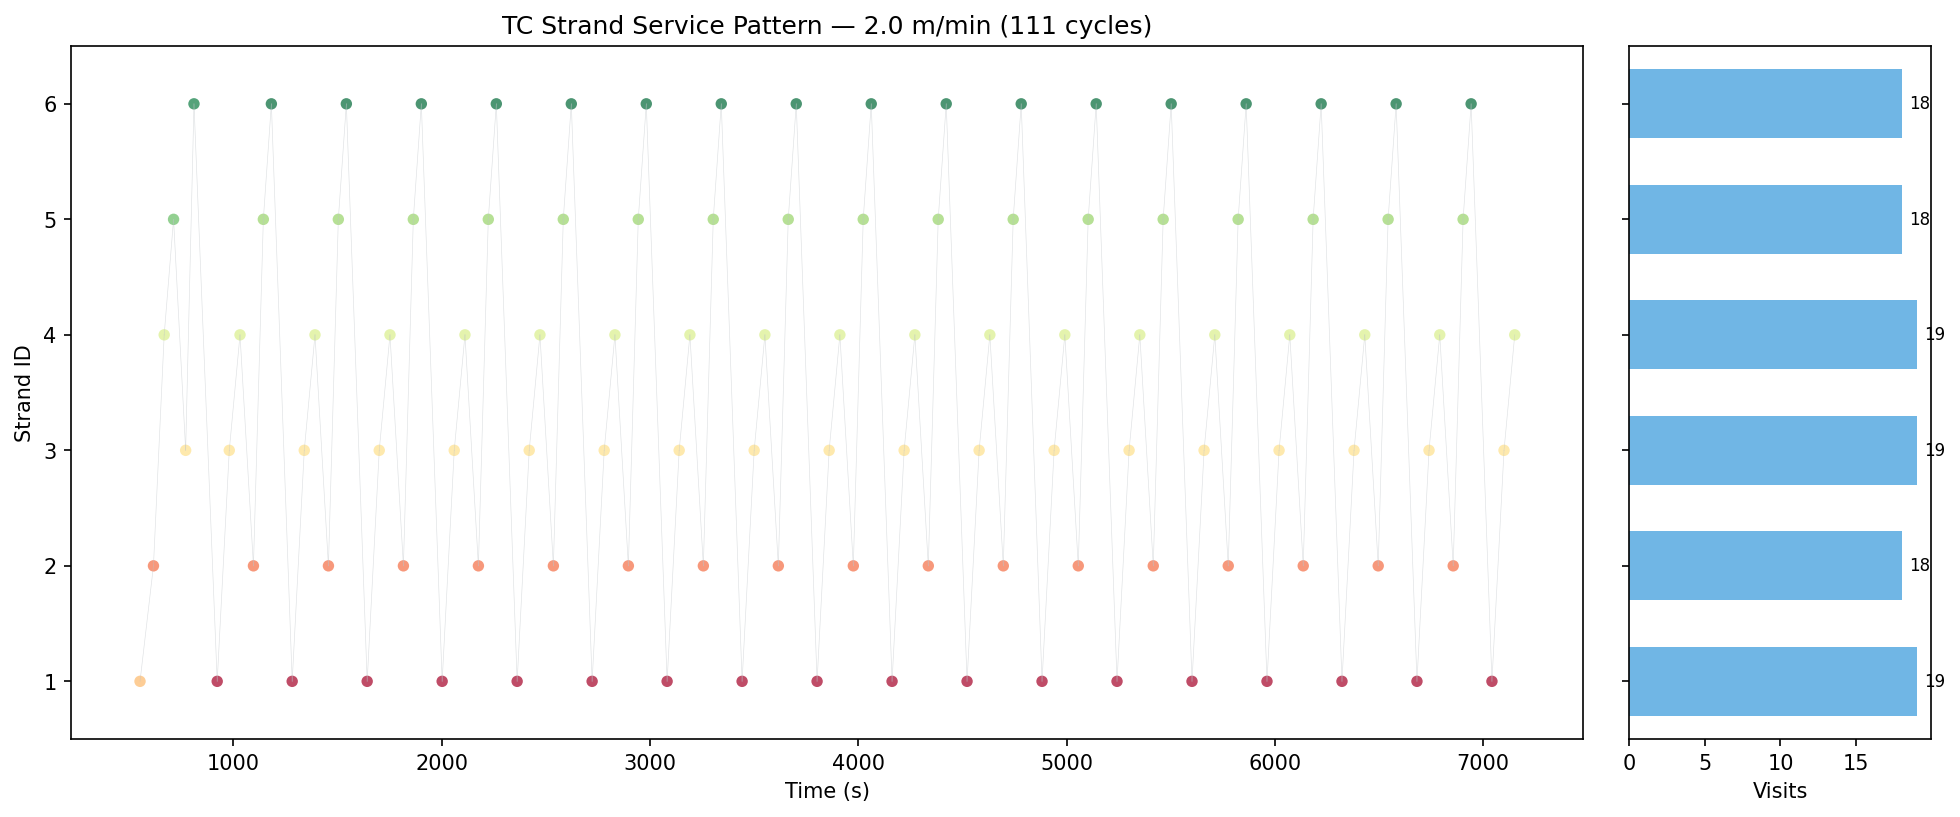
\includegraphics[width=0.85\textwidth]{output/v2.0/V2_tc_strand_pattern.png}
\caption{TC strand service pattern at $v = 2.0$\,m/min. Regular cyclic pattern; all 6 strands receive equitable service.}
\label{fig:v2.0-tc-pattern}
\end{figure}

\begin{figure}[H]
\centering
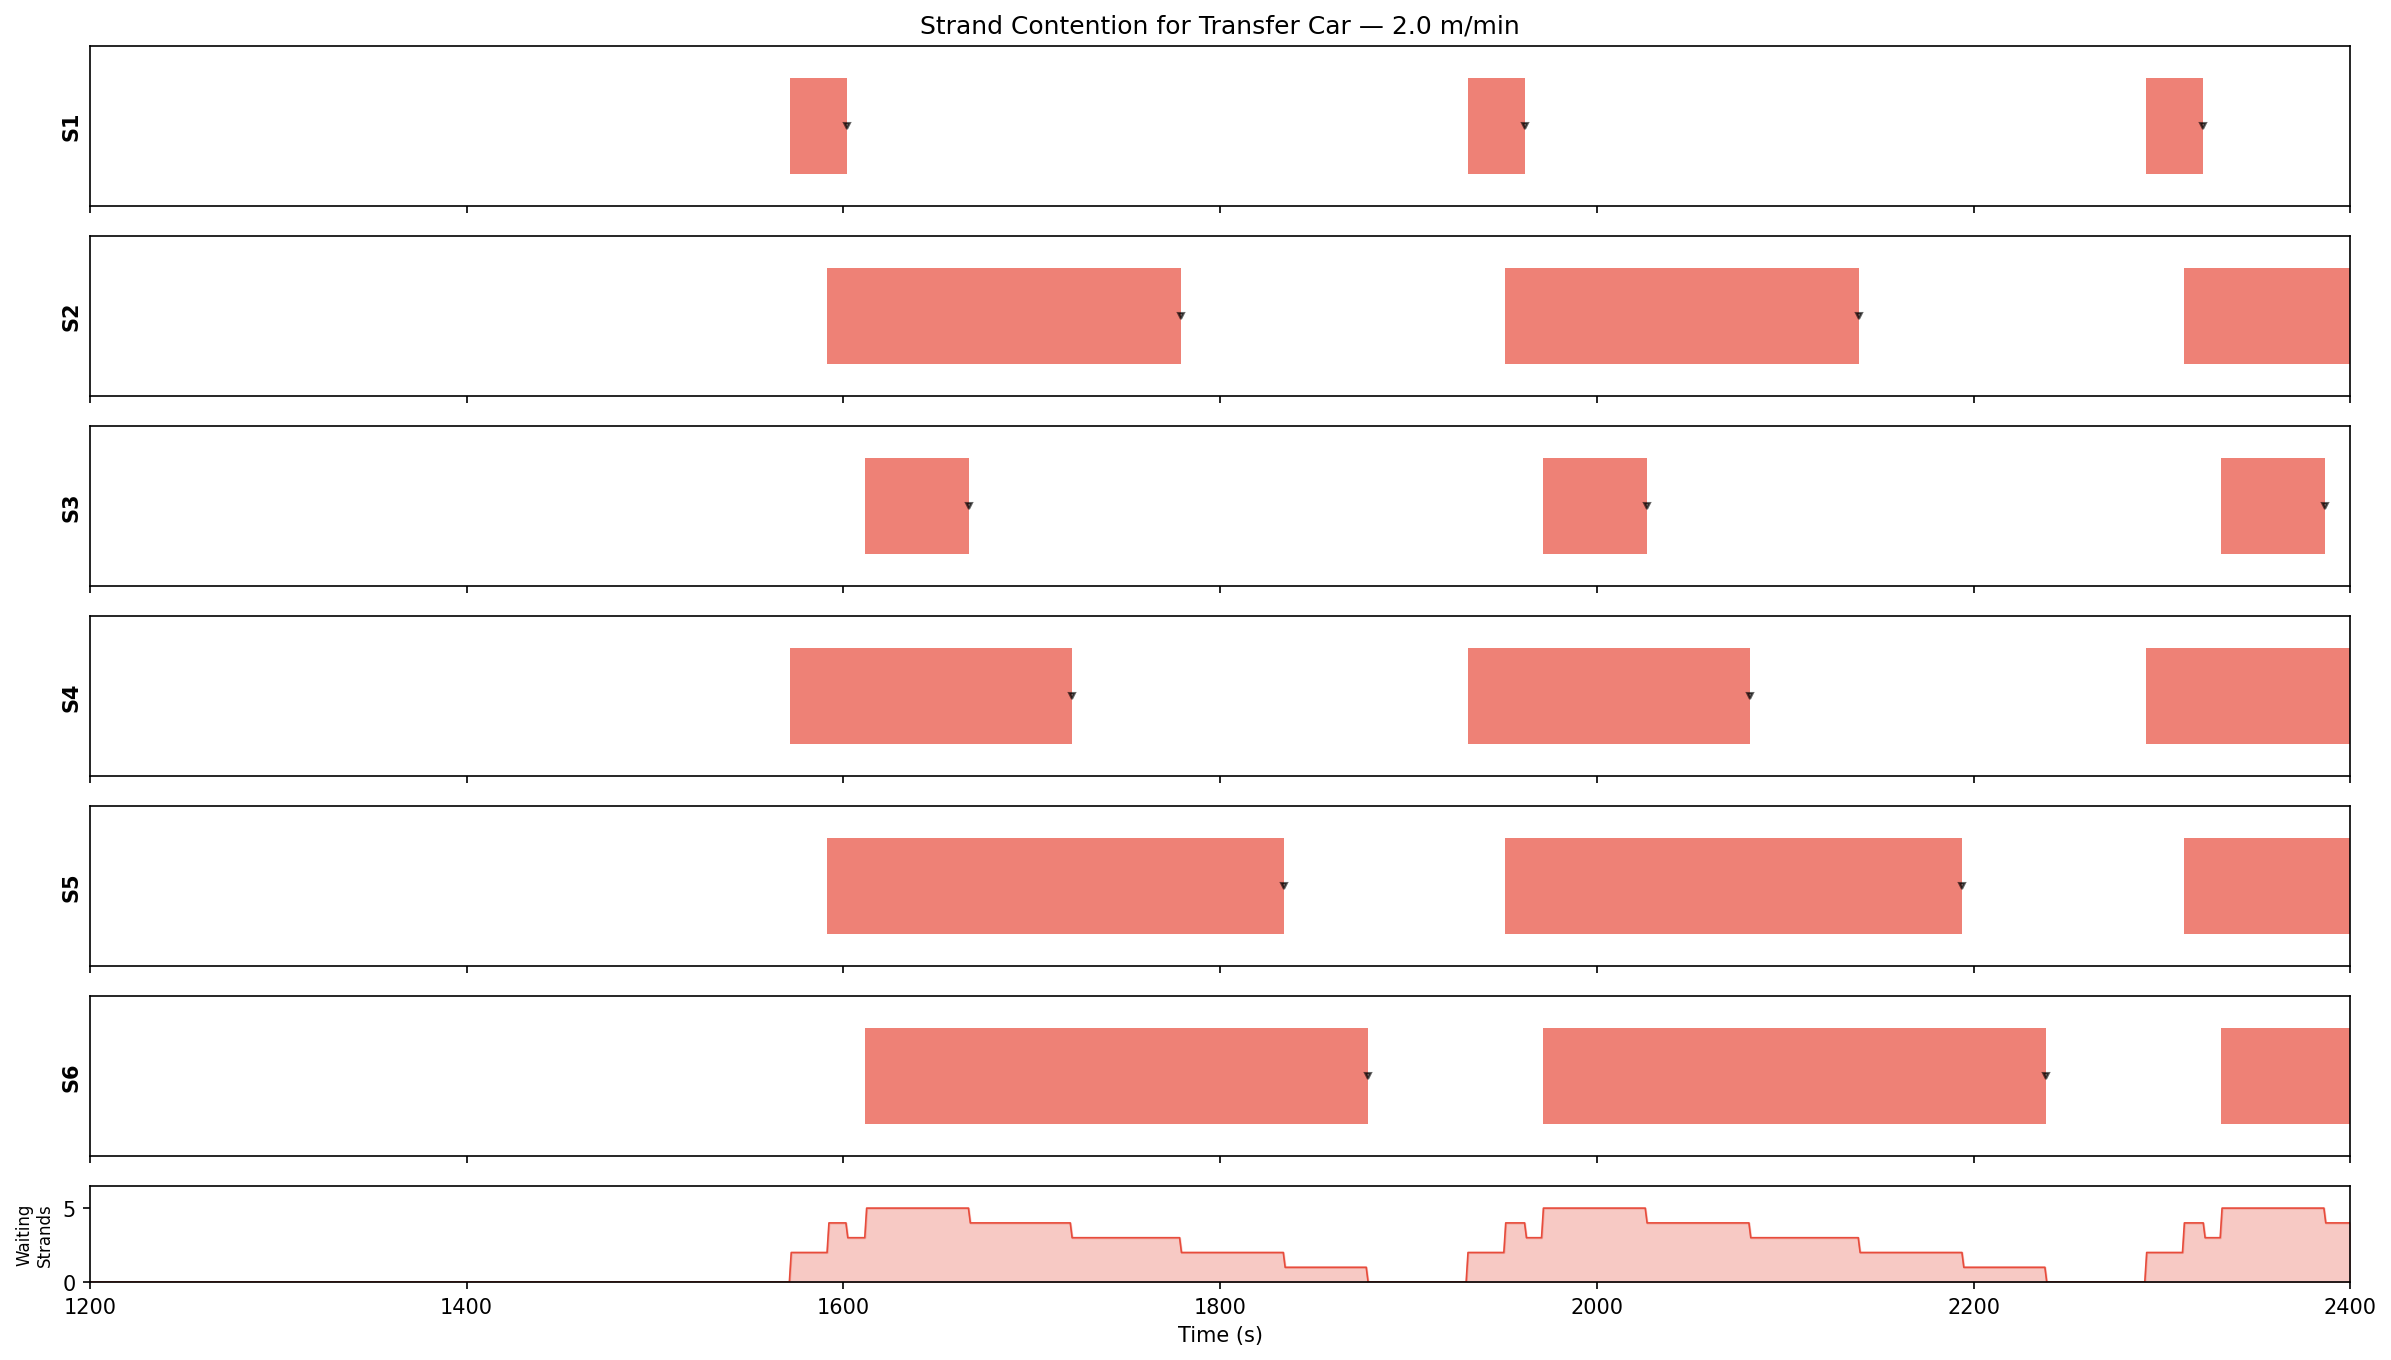
\includegraphics[width=0.85\textwidth]{output/v2.0/V7_strand_contention.png}
\caption{Strand contention at $v = 2.0$\,m/min. No overflow beyond pair buffer.}
\label{fig:v2.0-contention}
\end{figure}

\begin{figure}[H]
\centering
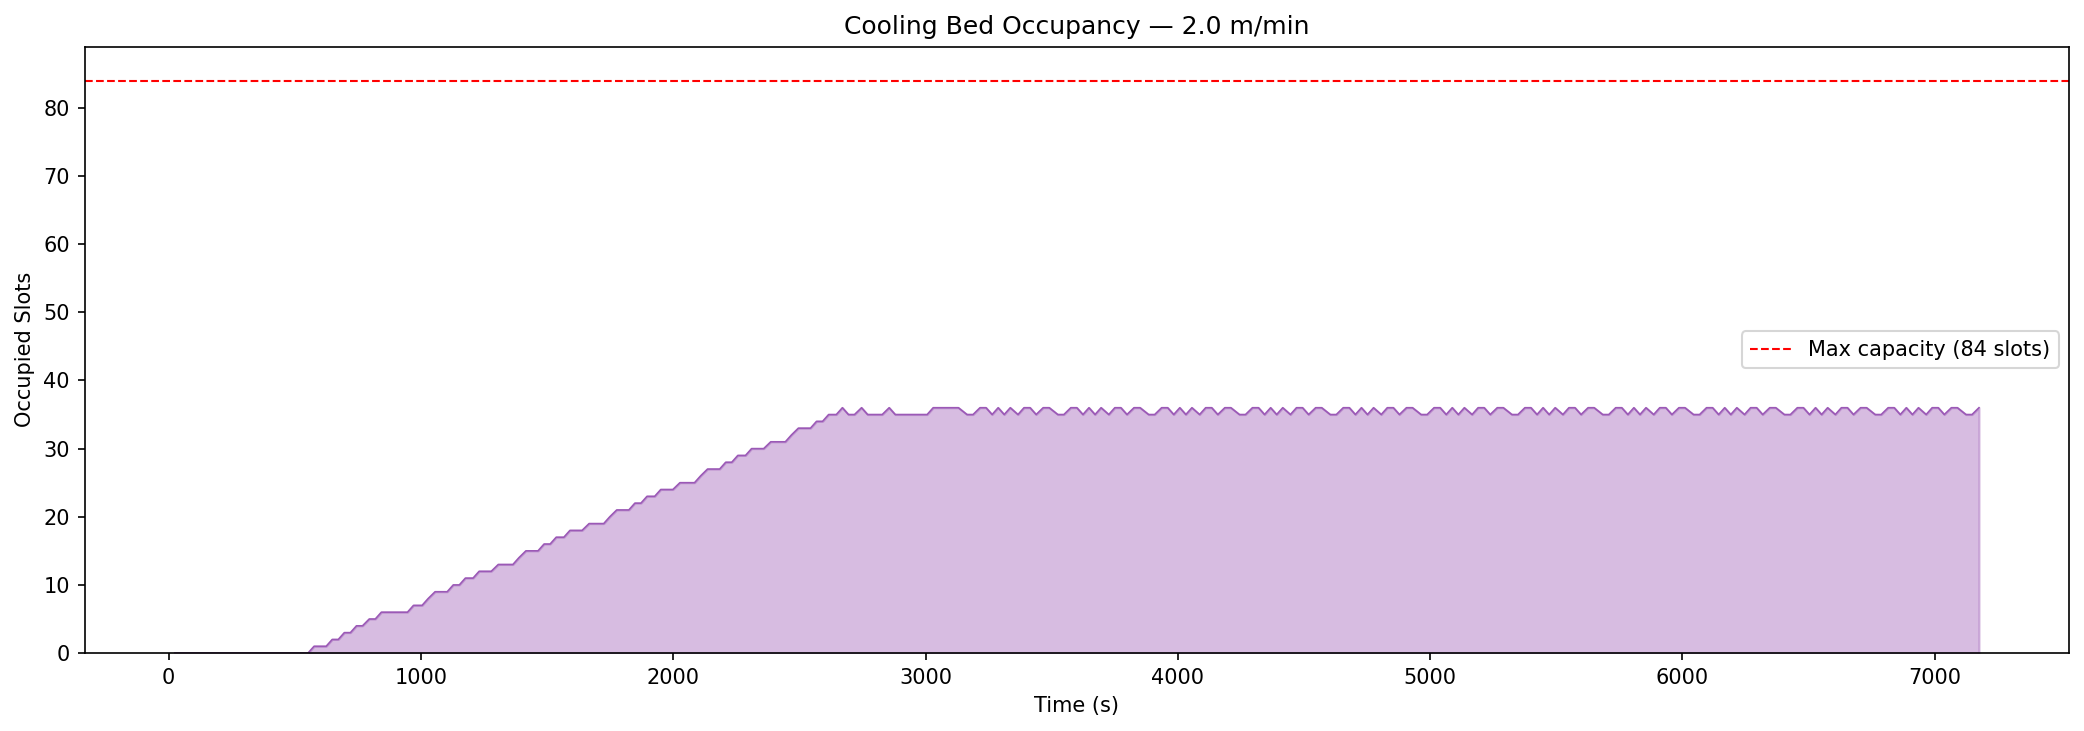
\includegraphics[width=0.85\textwidth]{output/v2.0/coolbed_occupancy.png}
\caption{Cooling bed occupancy at $v = 2.0$\,m/min. Steady state around 27 slots (32\% of 84). This means that at any given moment during steady-state operation, approximately 27 of the 84 slots contain a billet and 57 are empty. No risk of cooling bed overflow.}
\label{fig:v2.0-coolbed}
\end{figure}

%======================================================================
\section{Jammed Operating Point --- $v = 2.3$\,m/min}
\label{sec:jammed-point}

2.3\,m/min is the first tested velocity at which the system jams. The theoretical TC ceiling is 2.19\,m/min, so this operating point is 5\% above ceiling.

\subsection{Key Performance Indicators}

\begin{table}[H]
\centering
\caption{KPIs at $v = 2.3$\,m/min}
\label{tab:kpi-2.3}
\begin{tabular}{@{}lr@{}}
\toprule
Metric & Value \\
\midrule
Billets produced & 222 \\
Billets delivered to yard & 142 \\
Jam & YES --- strand 6, $t = 1236.5$\,s \\
TC utilization & 89.7\% \\
TC average cycle time & 59.6\,s \\
Avg wait for TC & 135.1\,s \\
Max wait for TC & 256.3\,s \\
Avg cooling bed occupancy & 25.9 slots \\
Max cooling bed occupancy & 34 slots \\
Primary bottleneck & TRAFFIC JAM (strand 6) \\
\bottomrule
\end{tabular}
\end{table}

\subsection{Failure Modes Explained}

Two distinct traffic jam mechanisms exist in the simulation. Both are detected only after the 1200\,s warmup period.

\textbf{Failure Mode 1: Discharge roller table collision (TC-limited)}

This is the primary failure mode. It occurs when the transfer car cannot serve all strands fast enough:
\begin{enumerate}
    \item Each strand produces a pair of billets every $720/v$ seconds (e.g., 313\,s at 2.3\,m/min).
    \item The TC needs 328.5\,s to visit all 6 strands (travel + hook operations).
    \item When $720/v < 328.5$ (i.e., $v > 2.19$\,m/min), the TC falls behind by $328.5 - 720/v$ seconds per cycle.
    \item As the TC falls behind, a strand's completed pair waits longer for pickup. The security stopper stays raised to hold the waiting pair.
    \item Meanwhile, the strand continues casting. A third billet arrives at the raised security stopper. This is the collision --- the simulation registers a traffic jam.
\end{enumerate}

At $v = 2.3$\,m/min, the per-cycle deficit is:
\begin{equation}
\text{deficit} = 328.5 - (720 / 2.3) = 328.5 - 313.0 = 15.5\;\text{s per cycle}
\end{equation}

Over approximately 4 cycles (from simulation start to warmup end), the accumulated deficit reaches approximately 60\,s. At $t = 1236.5$\,s (36.5\,s after warmup), strand~6 overflows.

\textbf{Failure Mode 2: Collecting table overflow (crane-limited)}

This occurs when the cranes cannot clear packs from the collecting table fast enough:
\begin{enumerate}
    \item Billets exit the cooling bed and are pushed into packs of 2 on the collecting table.
    \item The table holds a maximum of 7 packs.
    \item With grab-type crane (1 pack per trip, 274\,s cycle time), each crane clears 1 pack every 274\,s.
    \item Two cranes together clear 2 packs per 274\,s $= 0.00730$ packs/s.
    \item If the billet arrival rate exceeds the crane clearing rate, packs accumulate until the table is full.
    \item When pack~8 would be placed on a full table, the simulation registers a traffic jam.
\end{enumerate}

This mode is the binding constraint with realistic grab-type crane at velocities above 0.88\,m/min for 6 strands (see Section~\ref{sec:crane-bottleneck}).

\subsection{Why Strand 6 Jams First (at $v = 2.3$\,m/min)}

Strand~6 jams first because of the deterministic lag pattern. Strand~6 has a 40\,s startup lag (A1). Combined with the TC's round-robin service order, strand~6 is the strand where the accumulated TC deficit causes the third billet to arrive at the security stopper first. Different lag patterns or velocities may cause different strands to jam first (strand~2 jams first at $v = 2.6$ and 3.0\,m/min).

\subsection{TC Margin (Negative)}

\begin{equation}
\text{TC margin} = \frac{720}{2.3} - 328.5 = 313.0 - 328.5 = -15.5\;\text{s}
\end{equation}

A negative margin means sustained operation is mathematically impossible.

\subsection{Comparison: $v = 2.0$ vs $v = 2.3$}

\begin{table}[H]
\centering
\caption{Comparison of safe vs jammed operating points}
\label{tab:compare-2.0-2.3}
\begin{tabular}{@{}lrrr@{}}
\toprule
Metric & $v = 2.0$ & $v = 2.3$ & Change \\
\midrule
Jam & No & Yes ($t{=}1236.5$\,s) & --- \\
TC utilization & 86.1\% & 89.7\% & $+3.6$\,pp \\
TC avg cycle & 55.7\,s & 59.6\,s & $+3.9$\,s \\
TC margin & $+31.5$\,s & $-15.5$\,s & $-47.0$\,s \\
Billets produced & 228 & 222 & $-6$ \\
Max CB occupancy & 36 & 34 & $-2$ \\
\bottomrule
\end{tabular}
\end{table}

\textbf{Side-by-side plot comparisons:}

\begin{figure}[H]
\centering
\begin{minipage}{0.48\textwidth}
\centering
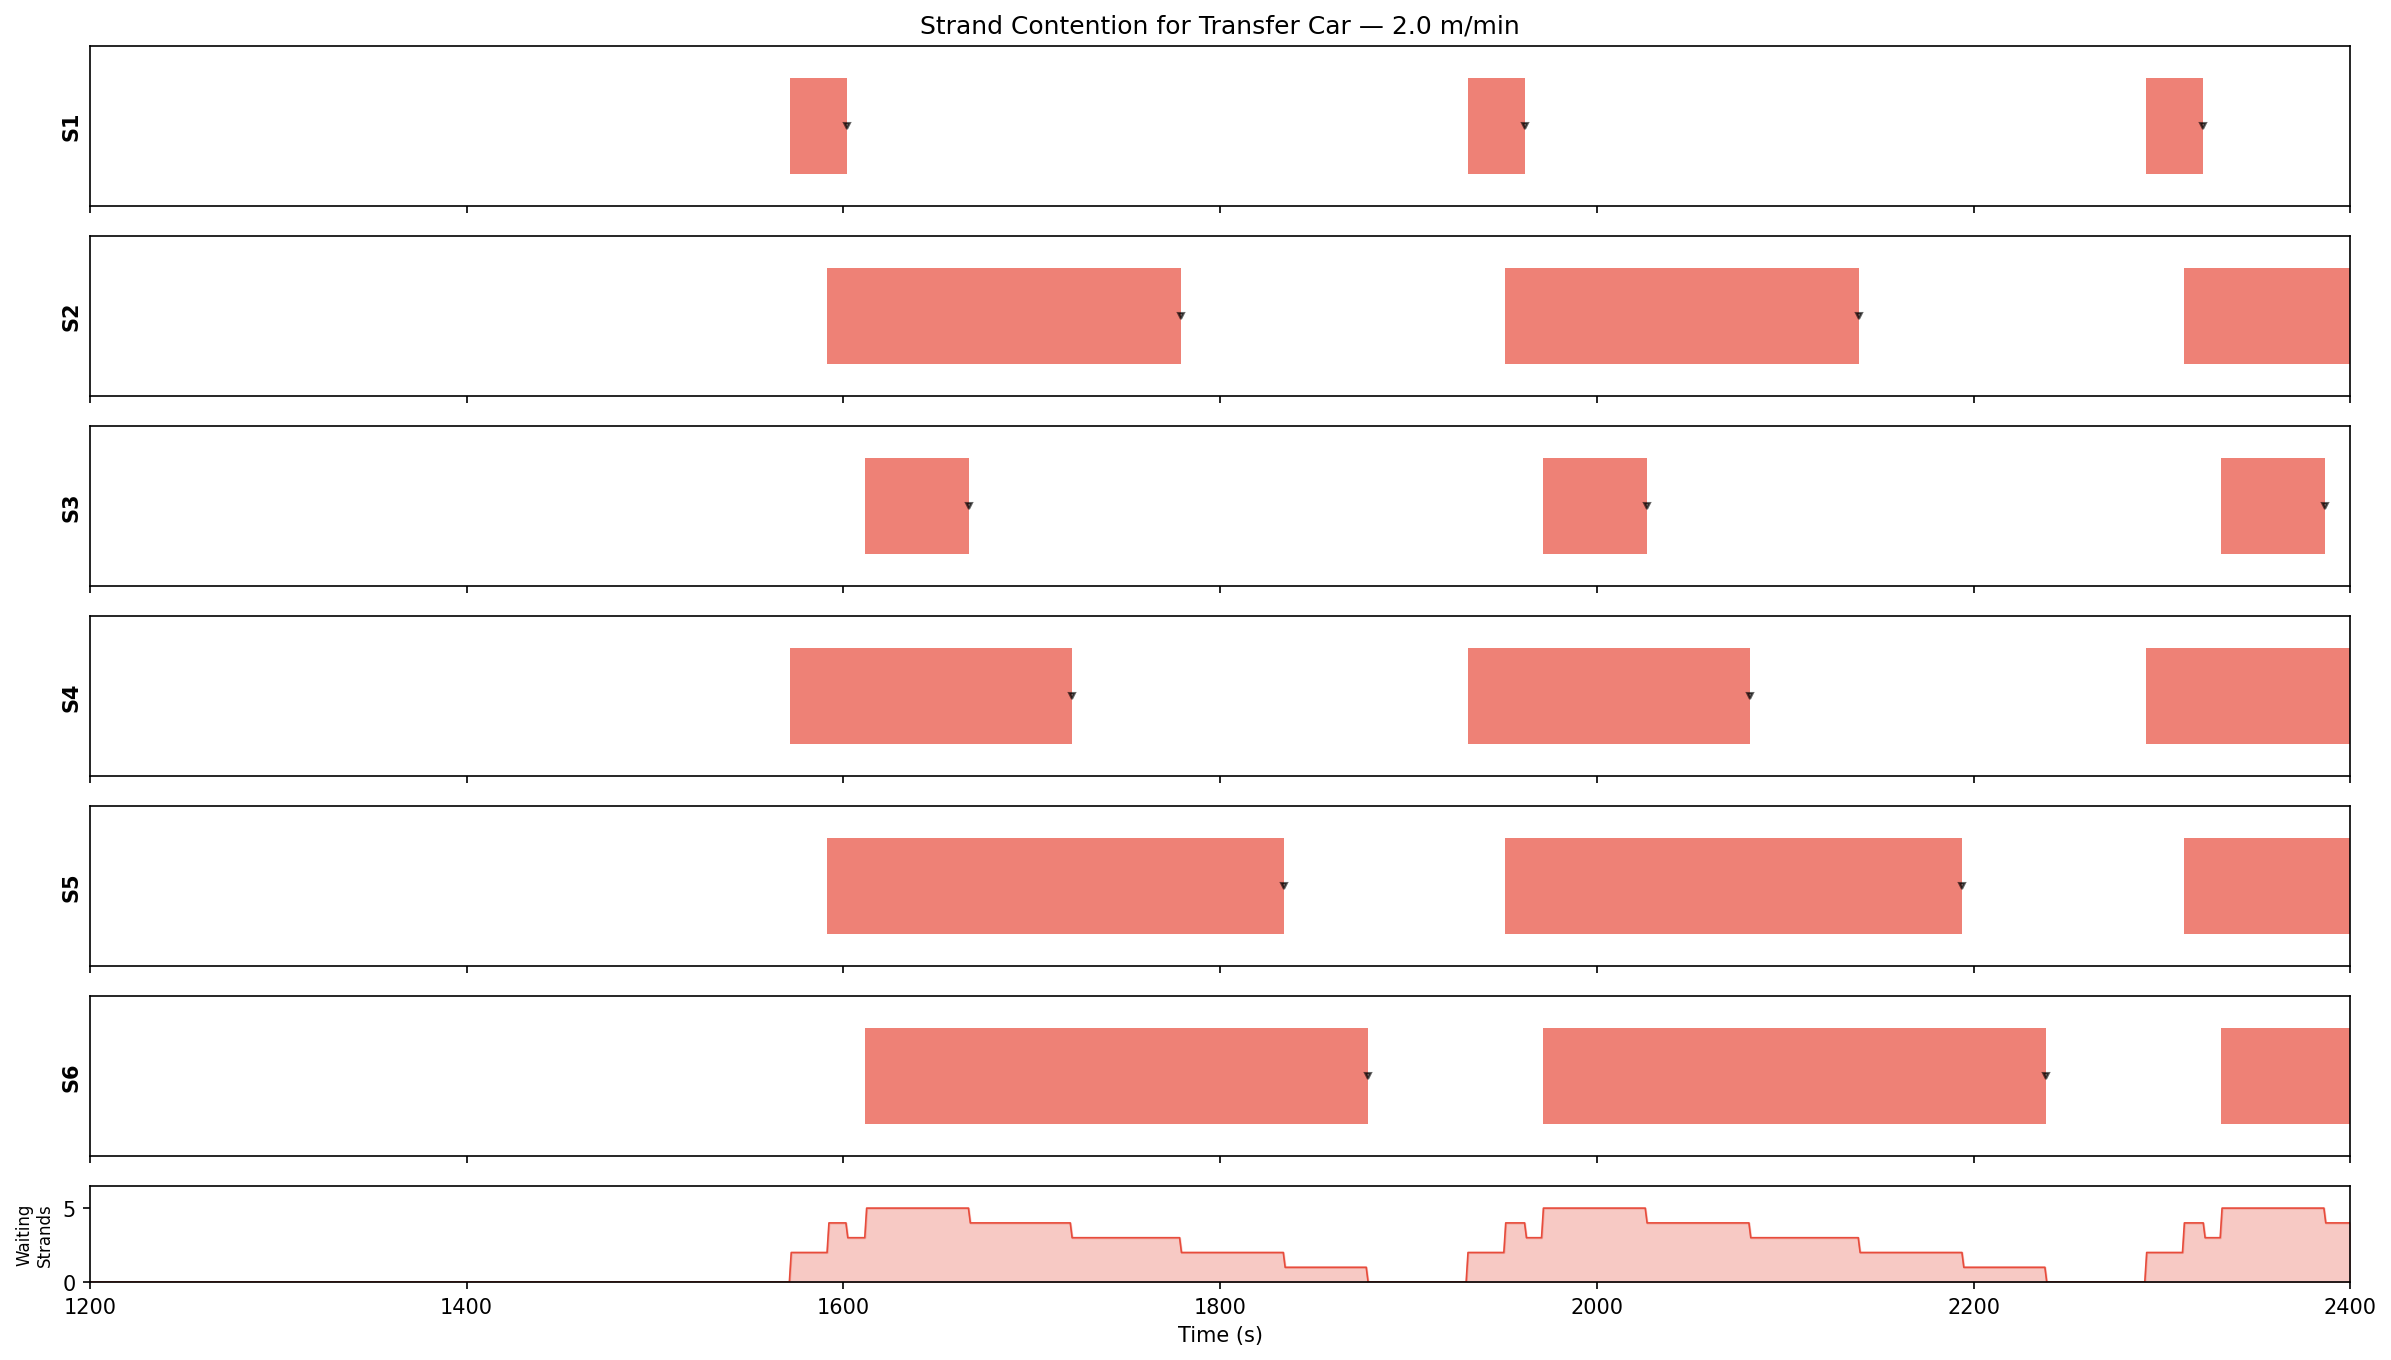
\includegraphics[width=\textwidth]{output/v2.0/V7_strand_contention.png}
\caption*{$v = 2.0$ --- No contention overflow}
\end{minipage}
\hfill
\begin{minipage}{0.48\textwidth}
\centering
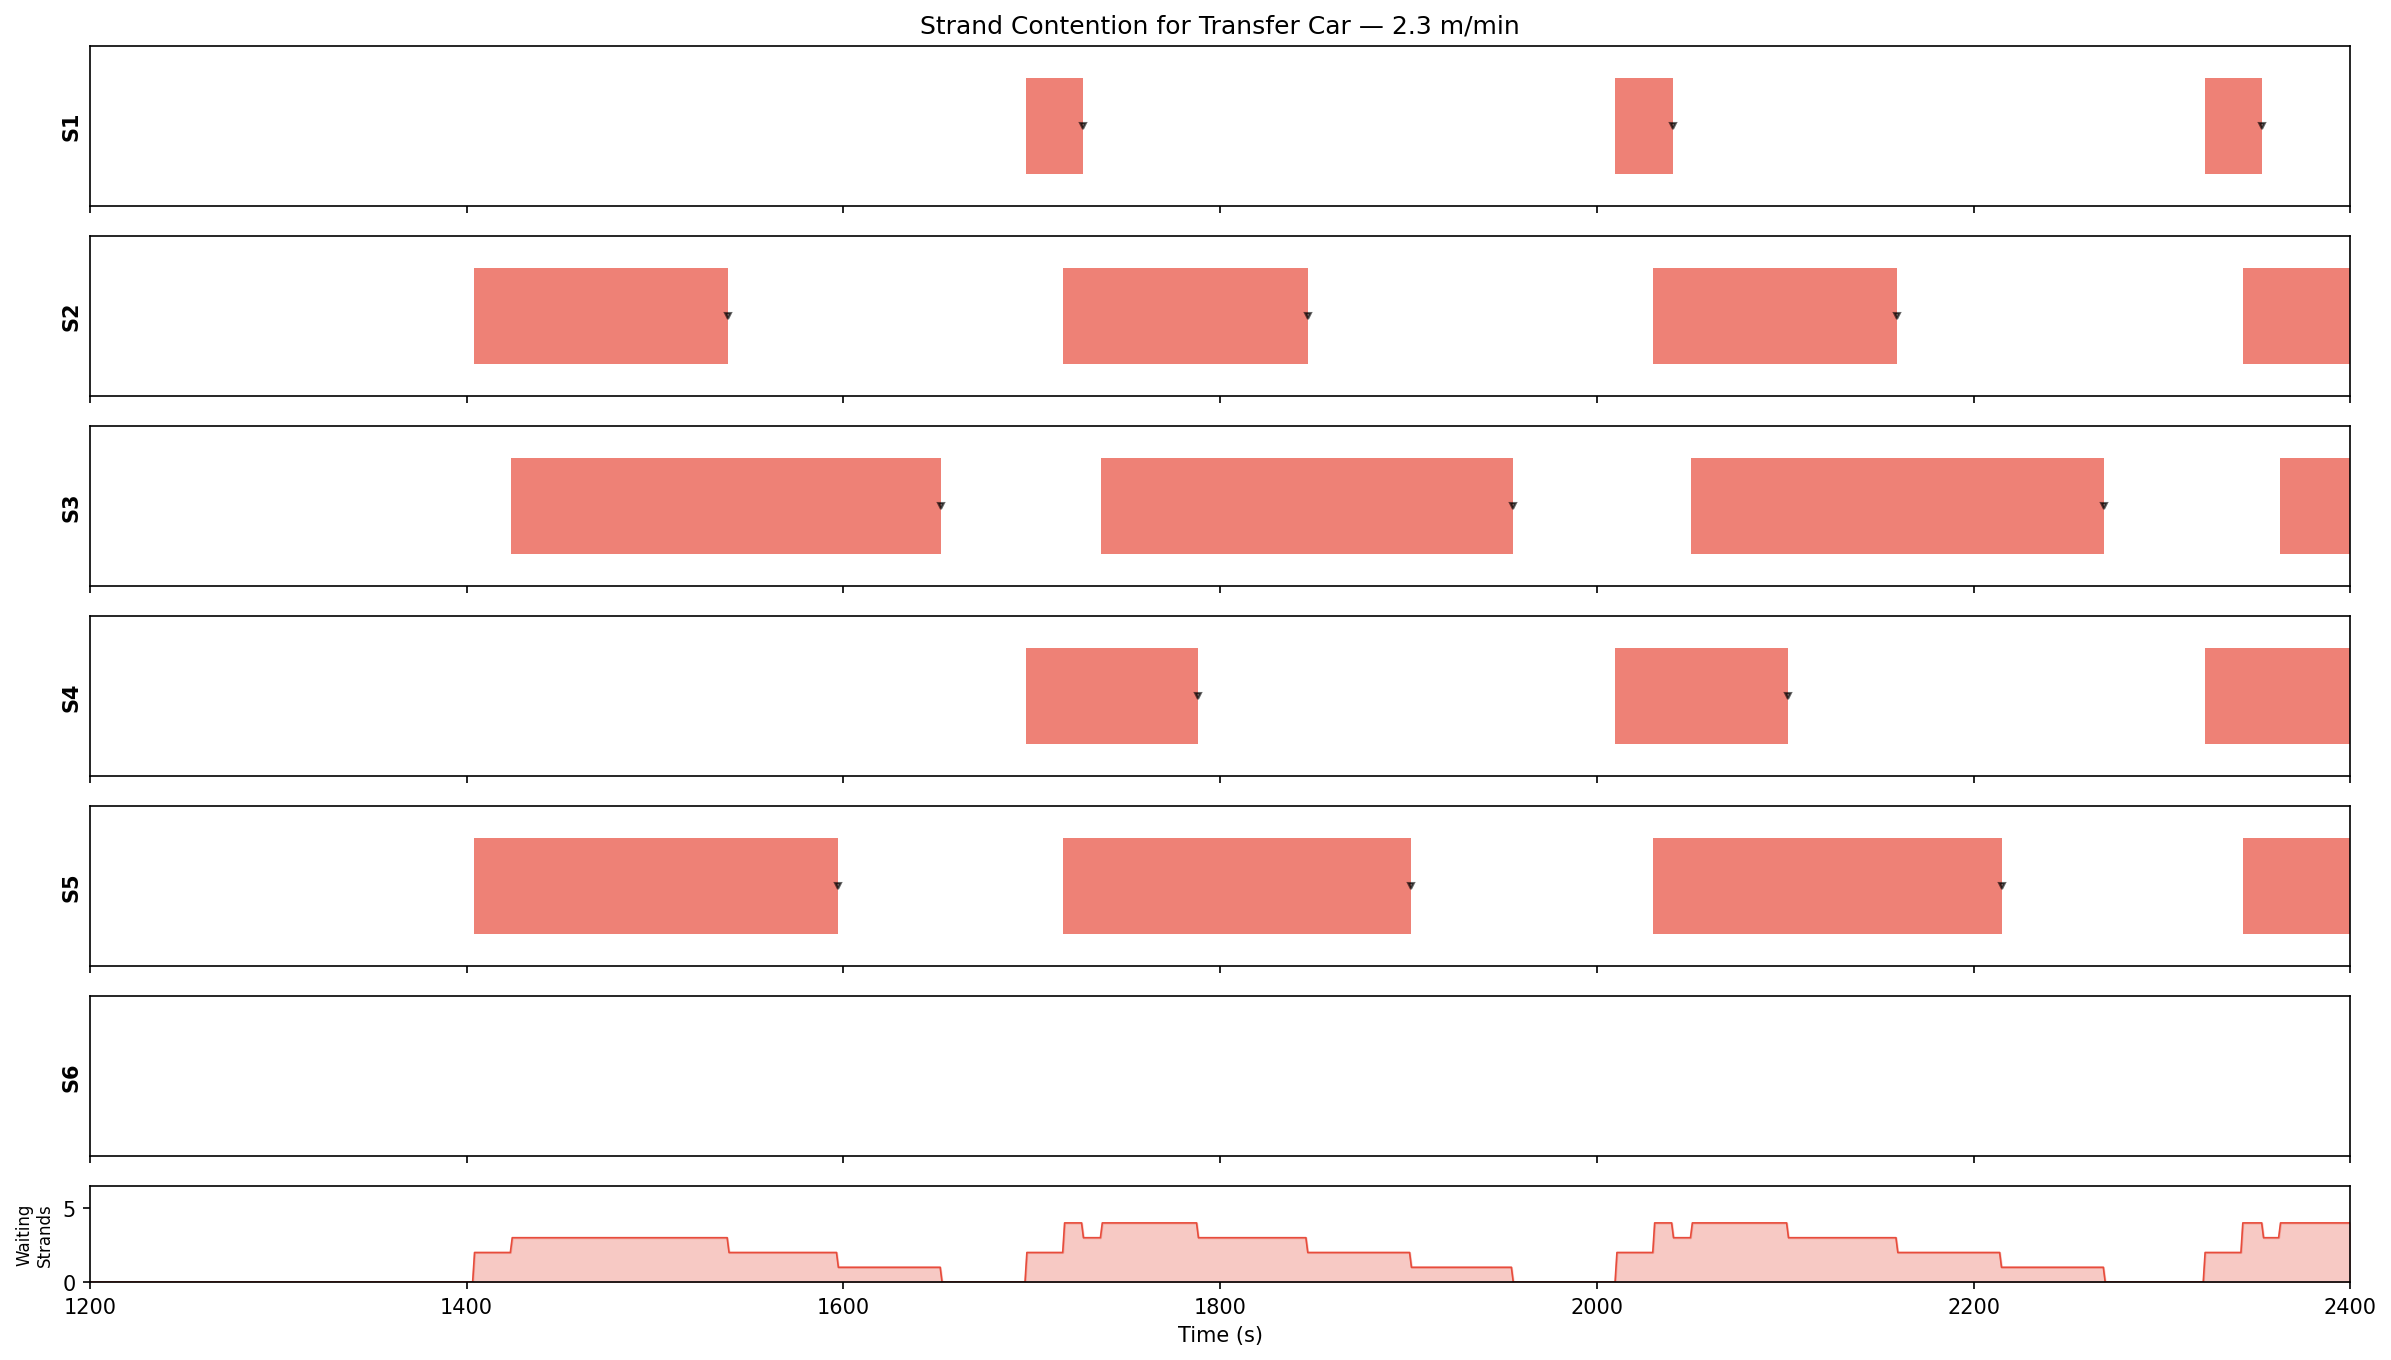
\includegraphics[width=\textwidth]{output/v2.3/V7_strand_contention.png}
\caption*{$v = 2.3$ --- Contention builds on strand 6}
\end{minipage}
\captionof{figure}{Strand contention comparison}
\label{fig:contention-compare}
\end{figure}

\begin{figure}[H]
\centering
\begin{minipage}{0.48\textwidth}
\centering
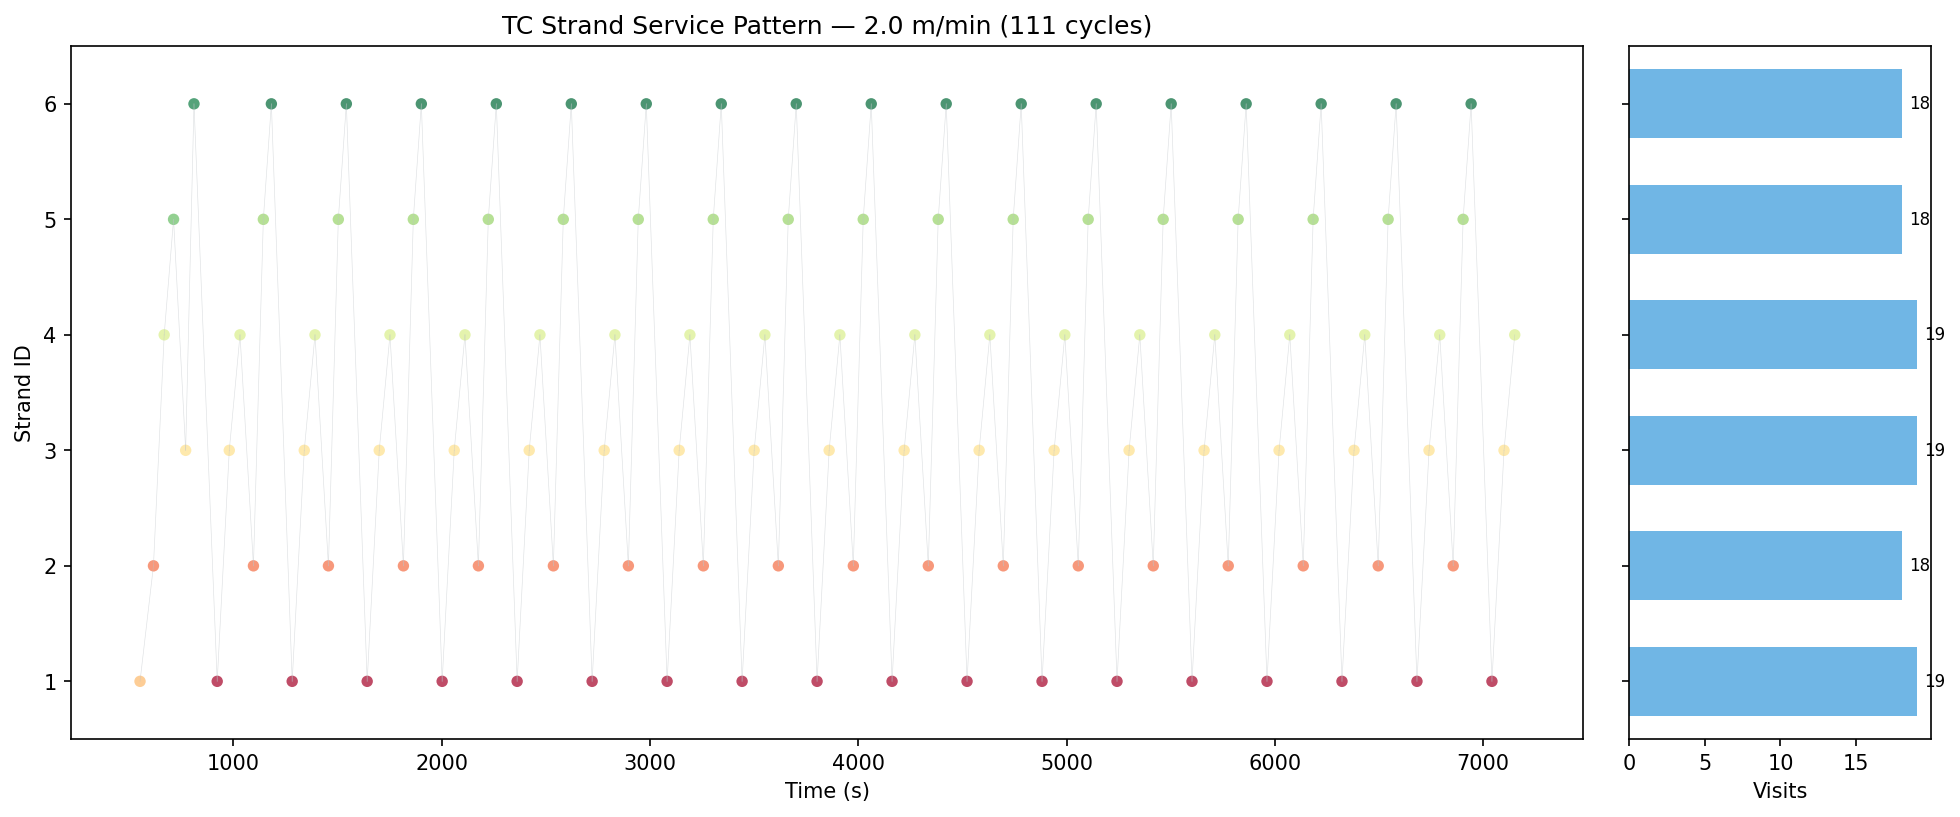
\includegraphics[width=\textwidth]{output/v2.0/V2_tc_strand_pattern.png}
\caption*{$v = 2.0$ --- Regular service}
\end{minipage}
\hfill
\begin{minipage}{0.48\textwidth}
\centering
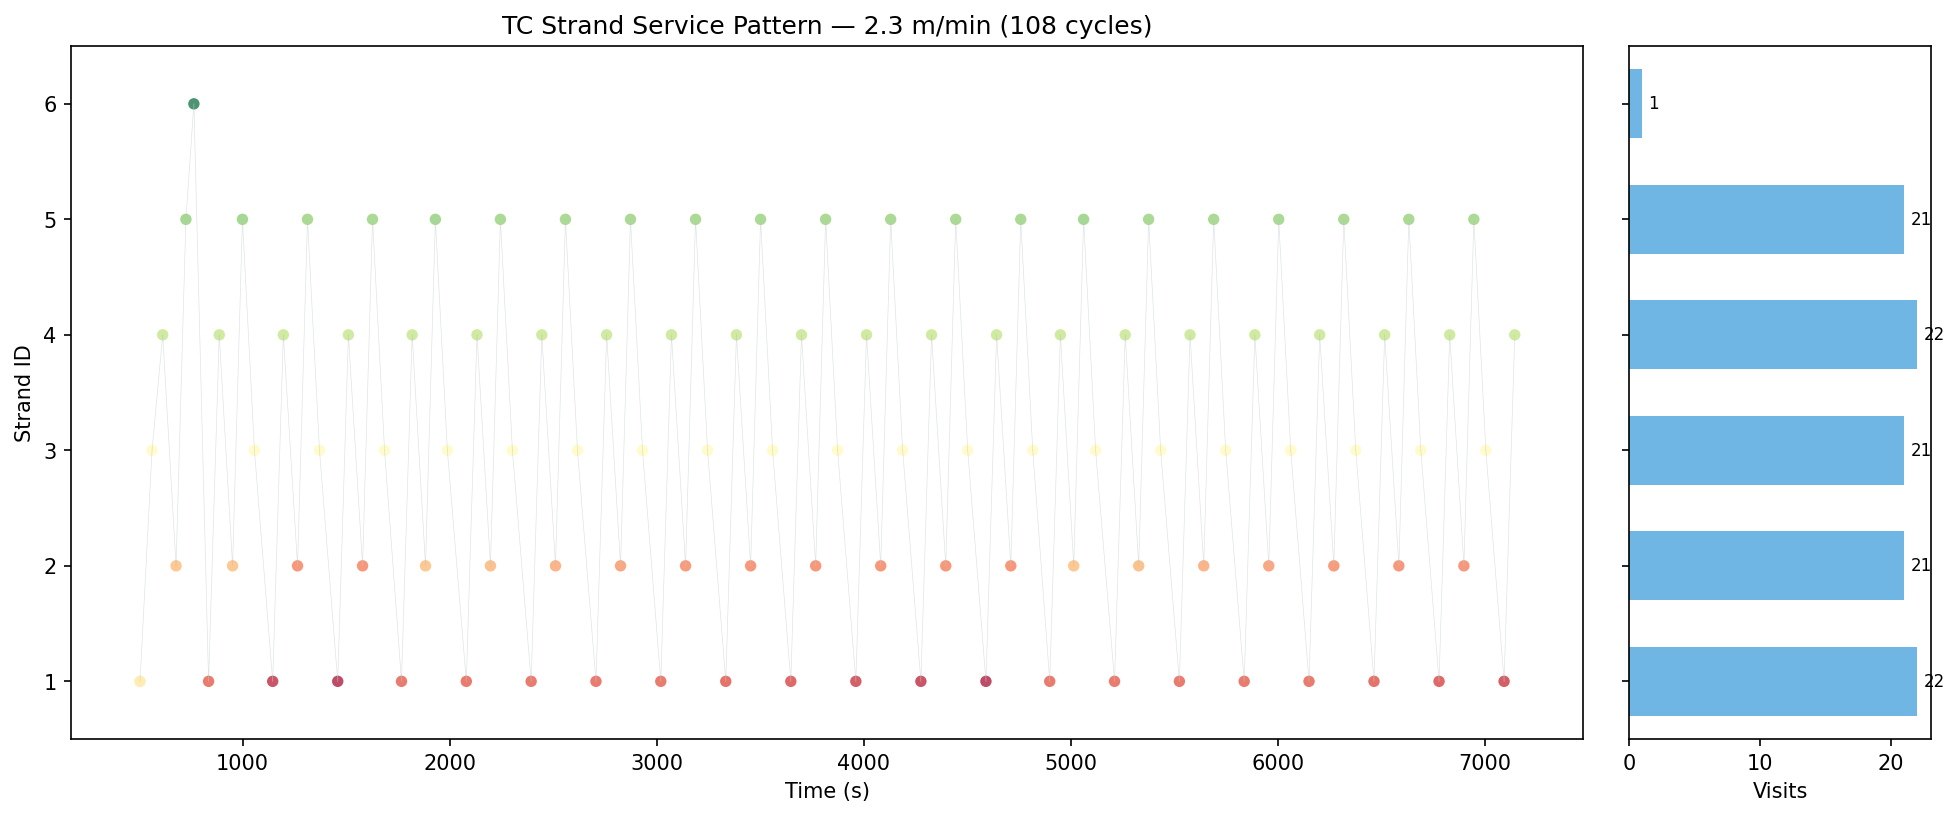
\includegraphics[width=\textwidth]{output/v2.3/V2_tc_strand_pattern.png}
\caption*{$v = 2.3$ --- TC falls behind}
\end{minipage}
\captionof{figure}{TC strand service pattern comparison}
\label{fig:tc-pattern-compare}
\end{figure}

%======================================================================
\section{Further Jammed Cases --- $v = 2.6$, 3.0\,m/min}
\label{sec:further-jams}

\begin{table}[H]
\centering
\caption{Progression of jammed cases}
\label{tab:jam-progression}
\begin{tabular}{@{}lrrr@{}}
\toprule
Metric & $v = 2.3$ & $v = 2.6$ & $v = 3.0$ \\
\midrule
Jam time (s) & 1236.5 & 1228.5 & 1200.8 \\
Jam strand & 6 & 2 & 2 \\
TC margin (s) & $-15.5$ & $-51.5$ & $-88.5$ \\
Billets produced & 222 & 158 & 128 \\
Billets delivered & 142 & 104 & 88 \\
TC utilization & 89.7\% & 65.2\% & 53.7\% \\
TC avg cycle (s) & 59.6 & 60.2 & 61.3 \\
Max CB occupancy & 34 & 27 & 24 \\
\bottomrule
\end{tabular}
\end{table}

\textbf{Key observations:}
\begin{itemize}
    \item Jam onset moves closer to warmup boundary. At $v = 3.0$\,m/min, the jam occurs at $t = 1200.8$\,s --- barely 0.8\,s after warmup ends.
    \item TC utilization paradoxically drops at higher velocities because jams halt production early.
    \item Fewer billets are produced despite faster casting: 3.0\,m/min produces only 128 billets vs 228 at 2.0\,m/min (44\% fewer).
\end{itemize}

\subsection{Bottleneck Progression --- Wait Time Analysis}

\textbf{Definition of wait times:}
\begin{itemize}
    \item \textbf{Discharge wait (for TC):} Time a completed billet pair spends at the discharge stopper waiting for the transfer car to arrive and pick it up. Measured from the moment both billets in the pair reach their stoppers until the TC hooks are lowered.
    \item \textbf{TC wait:} Total time a billet waits at the discharge area, including both the time to form a pair and the time waiting for TC pickup.
\end{itemize}

\begin{table}[H]
\centering
\caption{Wait time progression across jammed cases}
\label{tab:bottleneck-progression}
\begin{tabular}{@{}crrrr@{}}
\toprule
Velocity & Avg Discharge (s) & Max Discharge (s) & Avg TC (s) & Max TC (s) \\
\midrule
2.3 & 51.8 & 133.7 & 135.1 & 256.3 \\
2.6 & 56.7 & 115.7 & 92.2 & 261.1 \\
3.0 & 44.8 & 97.2 & 88.1 & 271.6 \\
\bottomrule
\end{tabular}
\end{table}

\textbf{Why average wait times decrease at higher jammed velocities:} The jam occurs earlier (closer to warmup at 1200\,s), so fewer billets complete the full wait cycle before the simulation halts. The averages are computed over fewer data points, biased toward early billets that experienced shorter waits.

\textbf{Why maximum wait times remain similar (256--272\,s):} The maximum represents the worst-case billet --- the last one served before the jam. Regardless of velocity, the TC takes approximately the same per-strand cycle time ($54.75\;\text{s} \times 6 \approx 329$\,s for a full round), so the longest any billet can wait is roughly one full TC cycle.

%======================================================================
\section{Sub-Ceiling Operating Points --- $v = 1.5$, 1.8\,m/min}
\label{sec:sub-ceiling}

\begin{table}[H]
\centering
\caption{Sub-ceiling operating point results}
\label{tab:sub-ceiling}
\begin{tabular}{@{}lrrr@{}}
\toprule
Metric & $v = 1.5$ & $v = 1.8$ & $v = 2.0$ \\
\midrule
Billets produced & 168 & 204 & 228 \\
Billets delivered & 108 & 130 & 142 \\
Jam & No & No & No \\
TC utilization & 65.3\% & 77.6\% & 86.1\% \\
TC avg cycle (s) & 55.9 & 55.8 & 55.7 \\
TC margin (s) & $+151.5$ & $+71.5$ & $+31.5$ \\
TC margin (\%) & 46.1 & 18.1 & 9.6 \\
Avg wait TC (s) & 83.7 & 153.5 & 152.9 \\
Max wait TC (s) & 218.3 & 267.3 & 266.8 \\
Avg CB occupancy & 16.3 & 24.2 & 27.4 \\
Max CB occupancy & 23 & 32 & 36 \\
Avg table packs & 1.16 & 1.17 & 1.20 \\
Max table packs & 3 & 3 & 3 \\
\bottomrule
\end{tabular}
\end{table}

\textbf{Observations:}
\begin{itemize}
    \item TC cycle time is nearly constant across all jam-free velocities (55.7--55.9\,s), confirming cycle time is dominated by fixed travel distances and hook operations.
    \item Margin scales linearly with velocity: 151.5\,s at 1.5, 71.5\,s at 1.8, 31.5\,s at 2.0.
    \item \textbf{Cooling bed occupancy scales with throughput.} ``Average occupancy of 27.4 slots'' means: if you sampled the cooling bed at a random instant during the simulation, on average 27.4 out of 84 slots would contain a billet. The remaining 56.6 slots would be empty. This is computed by recording the slot count every cooling bed cycle (24\,s) and averaging over the full simulation. Values by velocity: 16.3 slots (1.5\,m/min), 24.2 slots (1.8\,m/min), 27.4 slots (2.0\,m/min). Even at 2.0\,m/min, the average is only 33\% of the 84-slot capacity, confirming the cooling bed is not a bottleneck.
    \item Collecting table never exceeds 3 packs (capacity = 7), confirming ample crane headroom.
\end{itemize}

\textbf{Recommended operating velocity:} $v = 1.8$\,m/min provides 18\% TC margin with productive throughput (204 billets per 2-hour simulation).

%======================================================================
\section{Velocity Sweep --- 20-Seed Monte Carlo}
\label{sec:sweep}

\textbf{Note:} The sweep in this section uses a crane configuration of 7 packs/trip to isolate the transfer car bottleneck. With the realistic grab-type crane (1 pack/trip), the crane becomes the bottleneck at lower velocities --- see Section~\ref{sec:crane-bottleneck}.

\begin{figure}[H]
\centering
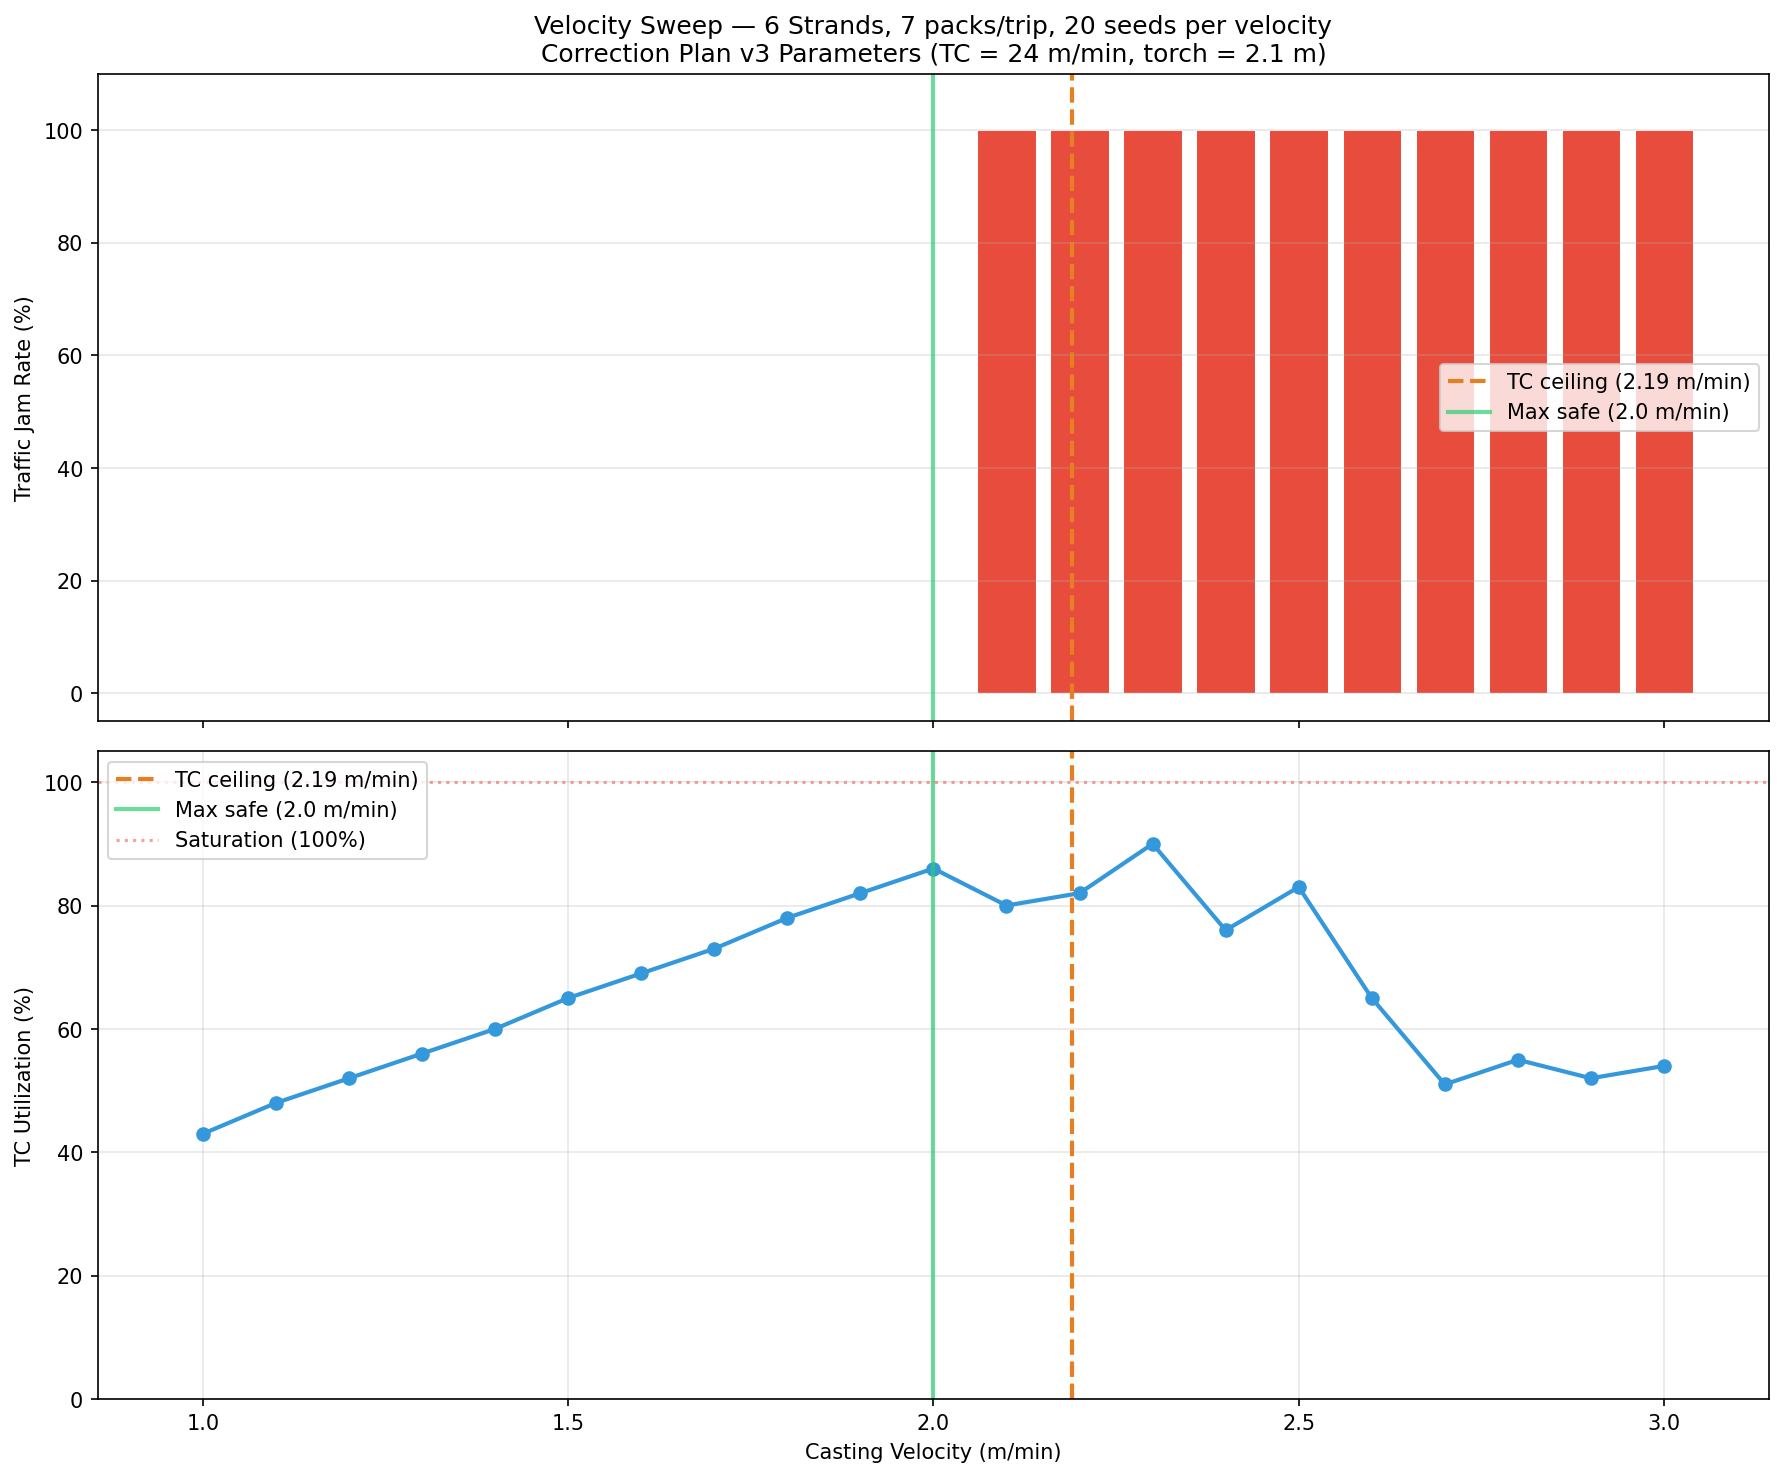
\includegraphics[width=0.85\textwidth]{output/velocity_sweep_20seeds.png}
\caption{Velocity sweep results (20 seeds per velocity). Sharp cliff at 2.0--2.1\,m/min.}
\label{fig:velocity-sweep}
\end{figure}

\subsection{What This Sweep Tests}

A ``velocity sweep'' means: run the full 7200\,s simulation at each velocity from 1.0 to 3.0\,m/min (in 0.1\,m/min steps). At each velocity, repeat the experiment 20 times with different random seeds. Count how many of the 20 runs produce a traffic jam. The \textbf{maximum safe velocity} is defined as the highest velocity where 0 out of 20 runs jammed.

\subsection{Results}

\begin{table}[H]
\centering
\caption{Velocity sweep jam rates}
\label{tab:sweep-results}
\begin{tabular}{@{}cl@{}}
\toprule
Velocity Range & Jam Rate \\
\midrule
1.0 -- 2.0\,m/min & 0\% (0/20 seeds) \\
2.1 -- 3.0\,m/min & 100\% (20/20 seeds) \\
\bottomrule
\end{tabular}
\end{table}

\textbf{Maximum safe velocity (TC-limited, 7 packs/trip crane): 2.0\,m/min.}

\subsection{Key Finding: Sharp Cliff Transition}

The transition from 0\% to 100\% jam rate occurs in a single 0.1\,m/min step between 2.0 and 2.1\,m/min. There is no gradual degradation --- no velocity produces partial jam rates (e.g., 50\% of seeds jamming).

\textbf{Why the cliff is sharp, not gradual:} The simulation uses deterministic strand lags (A1). The TC deficit per cycle is a fixed quantity at any given velocity --- it depends only on the TC travel distances and hook operation times, not on random seed. Either the margin is positive (the TC finishes serving all 6 strands before the next pair arrives --- no jam, regardless of seed) or negative (the TC structurally cannot keep up --- jam guaranteed, regardless of seed). The random seed affects only cooling bed and crane timing, which do not influence the TC bottleneck.

\subsection{Validation of TC Ceiling}

The theoretical TC ceiling is 2.19\,m/min. The sweep shows the operational maximum is 2.0\,m/min. The gap of 0.19\,m/min (8.7\%) arises from transient queuing effects: the TC does not always travel the average distance, sometimes arrives before pairs are ready, and has finite coordination overhead.

\subsection{Statistical Confidence}

With 20 seeds per velocity:
\begin{itemize}
    \item At 2.0\,m/min: 0/20 jams. 95\% CI: $[0\%, 16.8\%]$ (Clopper--Pearson).
    \item At 2.1\,m/min: 20/20 jams. 95\% CI: $[83.2\%, 100\%]$.
\end{itemize}

%======================================================================
\section{Crane Parametric Analysis}
\label{sec:crane-parametric}

This study varies the number of packs per crane trip (grab size) while keeping all other parameters at default (6 strands).

\begin{figure}[H]
\centering
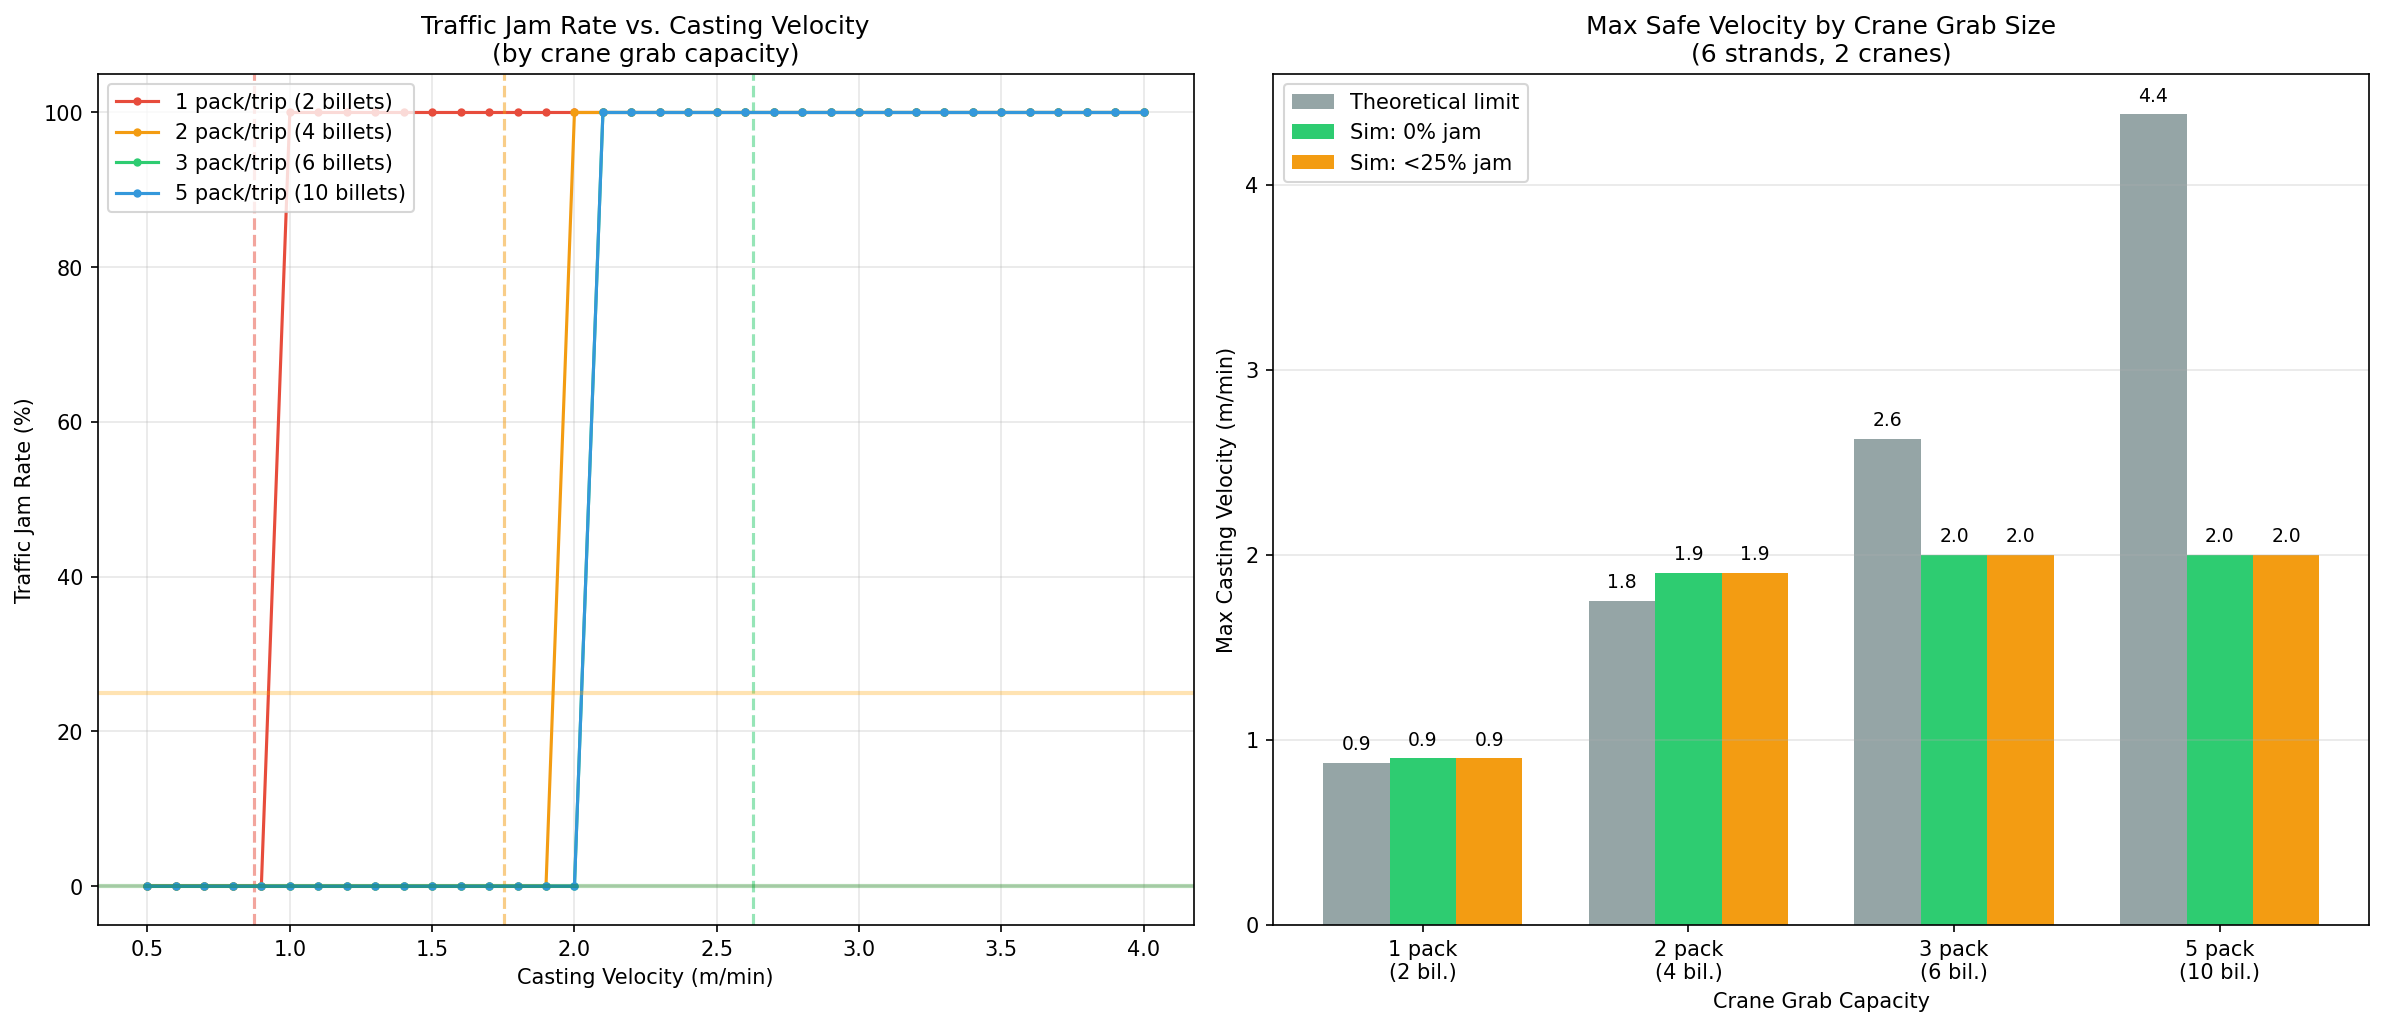
\includegraphics[width=0.85\textwidth]{output/crane_parametric_analysis.png}
\caption{Crane parametric analysis: max safe velocity vs grab size.}
\label{fig:crane-parametric}
\end{figure}

\begin{table}[H]
\centering
\caption{Crane parametric results (6 strands)}
\label{tab:crane-parametric}
\begin{tabular}{@{}ccc@{}}
\toprule
Packs/Trip & Max Safe Velocity & Limiting Factor \\
\midrule
1 & 0.9\,m/min & Crane \\
2 & 1.9\,m/min & Crane \\
3 & 2.0\,m/min & TC \\
5 & 2.0\,m/min & TC \\
\bottomrule
\end{tabular}
\end{table}

\textbf{Validation (1 pack/trip):}
\begin{equation}
v_\text{max} = \frac{1440 \times 1}{274 \times 6} = \frac{1440}{1644} = 0.88\;\text{m/min} \approx \text{sim's } 0.9\;\text{m/min}
\end{equation}

With $\geq 3$ packs/trip, the crane is no longer the bottleneck; the TC ceiling (2.0\,m/min operational) becomes the binding constraint.

\textbf{Practical implication:} With a grab-type crane (1 pack per trip), the crane is the bottleneck at 6 strands. The crane only stops being the bottleneck when the grab size reaches 3 packs per trip. Since the crane in this plant is grab-type and realistically picks up 1 pack of 2 billets per trip, the crane constraint is binding --- see Section~\ref{sec:crane-bottleneck} for the full analysis of practical options.

%======================================================================
\section{Strand $\times$ Crane Combined Parametric}
\label{sec:strand-crane}

\begin{figure}[H]
\centering
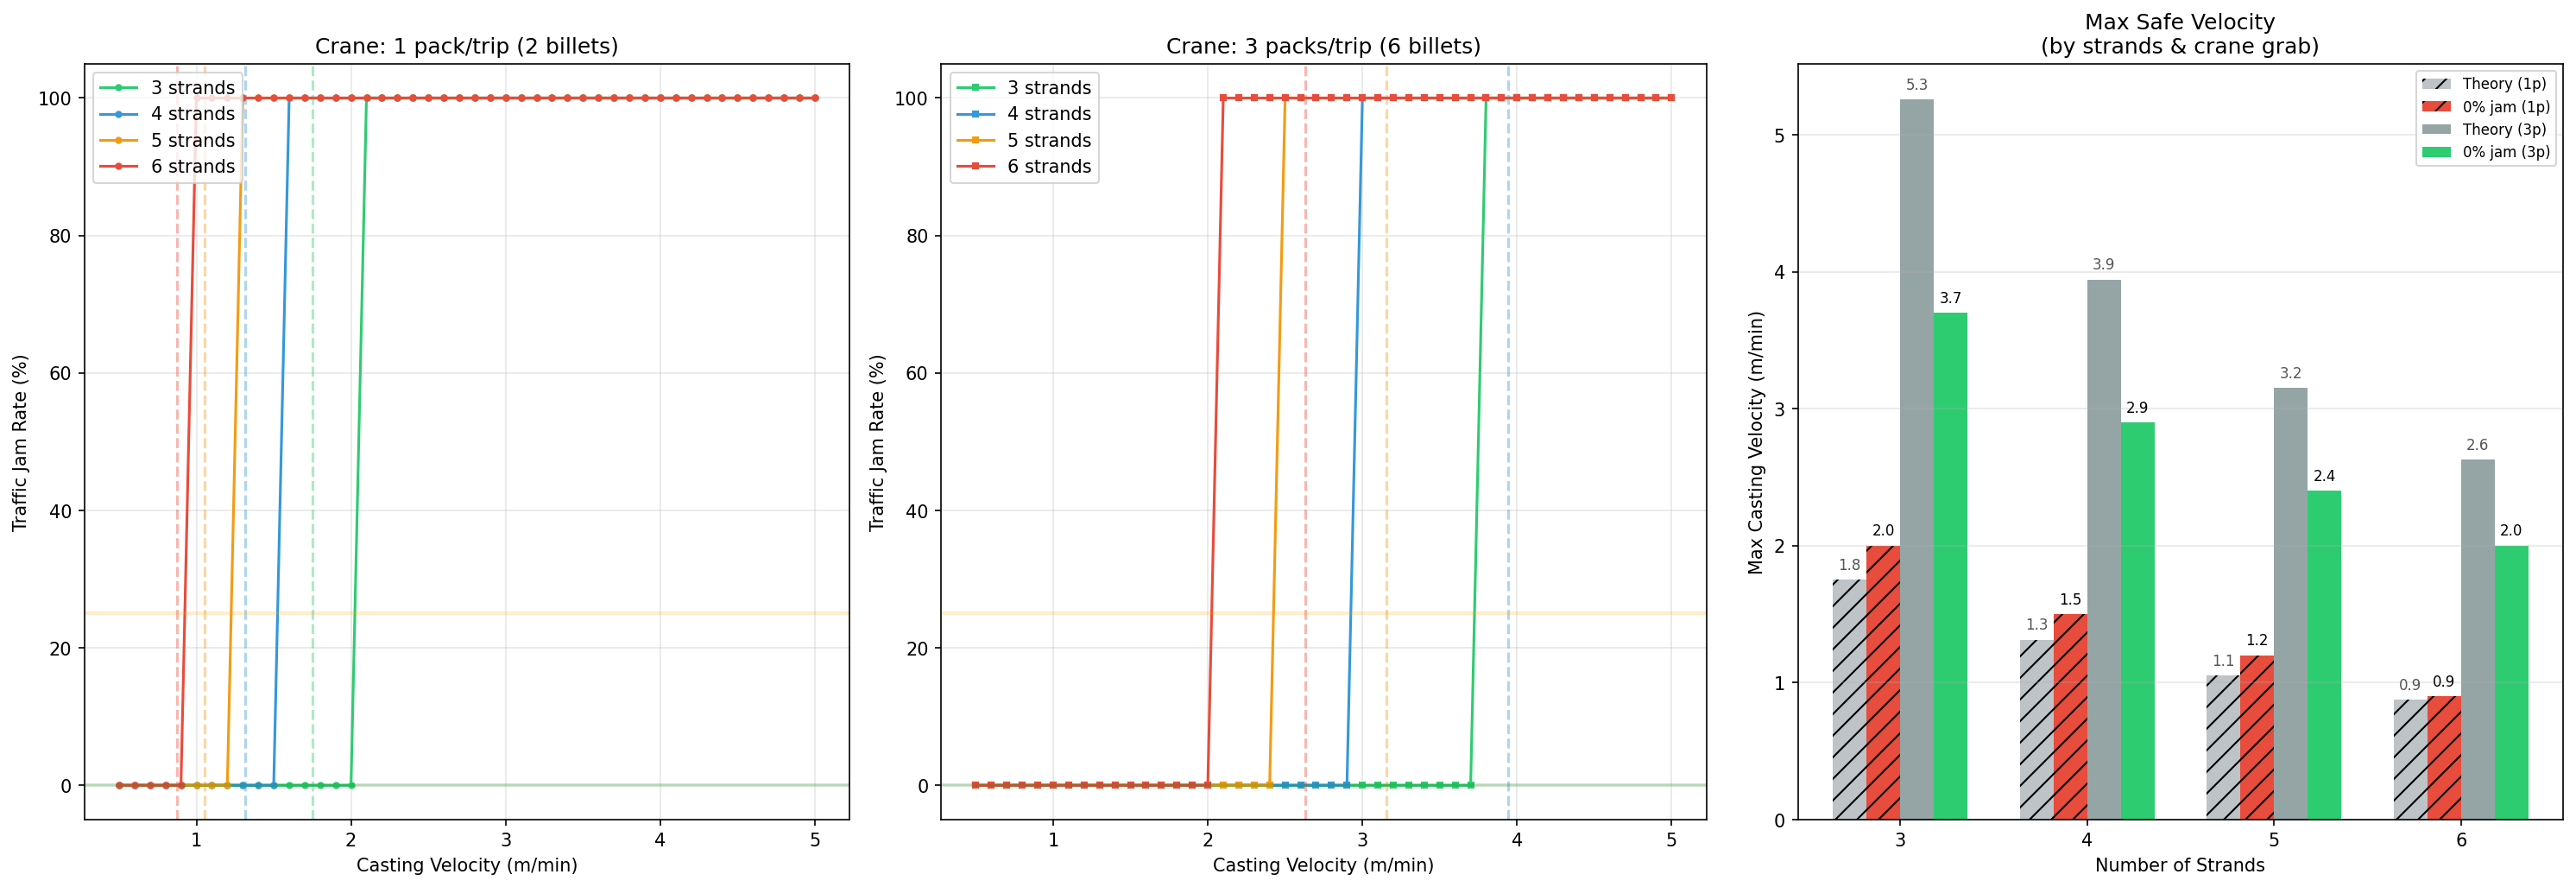
\includegraphics[width=0.85\textwidth]{output/strand_crane_parametric.png}
\caption{Combined strand count $\times$ crane grab size parametric.}
\label{fig:strand-crane}
\end{figure}

\begin{table}[H]
\centering
\caption{Maximum safe velocity (m/min) by strand count and crane grab size}
\label{tab:strand-crane}
\begin{tabular}{@{}ccccc@{}}
\toprule
Config & 3 Strands & 4 Strands & 5 Strands & 6 Strands \\
\midrule
1 pack/trip & 2.0 & 1.5 & 1.2 & 0.9 \\
3 packs/trip & 3.7 & 2.9 & 2.4 & 2.0 \\
\bottomrule
\end{tabular}
\end{table}

\textbf{Key insight:} Reducing strand count is the most effective lever. Going from 6 to 3 strands (with 3 packs/trip) increases the safe velocity from 2.0 to 3.7\,m/min --- an 85\% improvement.

For 3 strands with 3 packs/trip:
\begin{align}
T_\text{TC,3} &= 3 \times 54.75 = 164.25\;\text{s} \\
v_\text{max,TC} &= 720 / 164.25 = 4.38\;\text{m/min (theoretical)} \\
v_\text{max,crane} &= 1440 \times 3 / (274 \times 3) = 5.26\;\text{m/min}
\end{align}

The 3.7\,m/min simulation result is below both ceilings due to transient queuing effects.

%======================================================================
\section{Validation Summary}
\label{sec:validation}

\subsection{Quantitative Cross-Checks}

\begin{table}[H]
\centering
\caption{Simulation vs theory cross-checks}
\label{tab:validation}
\begin{tabular}{@{}lrrlp{4cm}@{}}
\toprule
Metric & Hand Calc & Simulation & Dev & Explanation \\
\midrule
TC avg cycle ($v{=}2.0$) & 54.75\,s & 55.7\,s & $+1.7\%$ & Queuing delay at strand \\
TC ceiling & 2.19\,m/min & 2.0\,m/min & $-8.7\%$ & Transient accumulation \\
Crane cycle (L1) & 274.0\,s & --- & --- & Consistent with config \\
Crane 1-pack limit & 0.88\,m/min & 0.9\,m/min & $+2.3\%$ & Discrete velocity step \\
Jam onset ($v{=}2.3$) & $>1200$\,s & 1236.5\,s & \checkmark & Post-warmup \\
Billets ($v{=}2.0$) & 240 & 228 & $-5.0\%$ & Warmup + lag offsets \\
\bottomrule
\end{tabular}
\end{table}

\subsection{Visual Validation}

\begin{enumerate}
    \item \textbf{Billet waterfall at $v = 2.0$} (\texttt{V6b\_multi\_billet\_waterfall.png}): Parallel strand cascades without overlap.
    \item \textbf{TC activity at $v = 2.0$} (\texttt{E2\_tc\_activity.png}): Round-robin pattern visiting all 6 strands cyclically.
    \item \textbf{Strand contention at $v = 2.3$} (\texttt{V7\_strand\_contention.png}): Progressive queue buildup on strand~6, consistent with deficit theory.
    \item \textbf{Cooling bed heatmap at $v = 2.0$} (\texttt{V4\_coolbed\_heatmap.png}): Sequential slot filling confirms walking beam behavior.
    \item \textbf{Wait distributions at $v = 2.0$} (\texttt{V3\_wait\_distributions.png}): Unimodal, consistent with single-bottleneck system.
    \item \textbf{Discharge timeline at $v = 2.0$} (\texttt{V1\_discharge\_timeline.png}): Regular events across all strands.
\end{enumerate}

%======================================================================
\section{Crane Bottleneck with Realistic Grab Constraints}
\label{sec:crane-bottleneck}

\subsection{Problem Statement}

The cranes are \textbf{grab-type} (not magnet). Each crane picks up \textbf{1 pack of 2 billets} per trip. The crane cycle time for layer~1 is 274.0\,s (see Section~\ref{sec:hand-calcs}).

With 2 cranes each picking 1 pack per trip, the maximum crane throughput is:
\begin{equation}
\text{crane\_supply} = \frac{2\;\text{packs}}{274.0\;\text{s}} = 0.00730\;\text{packs/s}
\end{equation}

At casting velocity $v$, 6 strands produce billets at a rate of:
\begin{align}
\text{billet\_rate} &= \frac{6 \times v}{6.0 \times 60} = \frac{v}{60}\;\text{billets/s} \\
\text{pack\_demand} &= \frac{\text{billet\_rate}}{2} = \frac{v}{120}\;\text{packs/s}\quad\text{(each pack = 2 billets)}
\end{align}

Setting supply $\geq$ demand:
\begin{equation}
\frac{2}{274} \geq \frac{v}{120} \quad\Rightarrow\quad v \leq \frac{2 \times 120}{274} = \frac{240}{274} = 0.876\;\text{m/min}
\end{equation}

For $N$ strands (generalised):
\begin{equation}
v_\text{max,crane} = \frac{1440}{N \times 274}
\end{equation}

\subsection{Simulation Results --- 1 Pack/Trip (Realistic Default)}

\begin{table}[H]
\centering
\caption{Crane bottleneck simulation results (1 pack/trip)}
\label{tab:crane-bottleneck}
\begin{tabular}{@{}ccccc@{}}
\toprule
Strands & Crane Ceiling (theory) & TC Ceiling (theory) & Binding Constraint & Max Safe Velocity (sim) \\
\midrule
6 & 0.88\,m/min & 2.19\,m/min & \textbf{Crane} & 0.9\,m/min \\
5 & 1.05\,m/min & 2.48\,m/min & \textbf{Crane} & 1.2\,m/min \\
4 & 1.31\,m/min & 2.94\,m/min & \textbf{Crane} & 1.5\,m/min \\
3 & 1.75\,m/min & 3.72\,m/min & \textbf{Crane} & 2.0\,m/min \\
\bottomrule
\end{tabular}
\end{table}

At every strand count, the crane is the bottleneck --- not the transfer car. Collecting table overflow occurs because cranes cannot clear packs fast enough, and the table fills to its 7-pack capacity.

\subsection{Practical Recommendations (Three Options)}

The reviewer identified three viable solutions. Here is the quantitative assessment of each:

\textbf{Option A: Reduce casting velocity (keep 6 strands, 1 pack/trip)}

Operate at $v \leq 0.8$\,m/min. This is conservative and may be too slow for production targets.

\textbf{Option B: Reduce strand count (keep 1 pack/trip)}

\begin{table}[H]
\centering
\caption{Strand reduction options with 1 pack/trip crane}
\label{tab:strand-reduction}
\begin{tabular}{@{}ccc@{}}
\toprule
Strands & Max Safe Velocity & Annual Throughput (est.) \\
\midrule
6 & 0.9\,m/min & $0.9 \times 6 = 5.4$\;strand$\cdot$m/min \\
5 & 1.2\,m/min & $1.2 \times 5 = 6.0$\;strand$\cdot$m/min \\
4 & 1.5\,m/min & $1.5 \times 4 = 6.0$\;strand$\cdot$m/min \\
3 & 2.0\,m/min & $2.0 \times 3 = 6.0$\;strand$\cdot$m/min \\
\bottomrule
\end{tabular}
\end{table}

Reducing from 6 to 5 strands increases total output from 5.4 to 6.0\;strand$\cdot$m/min despite casting fewer strands. Further reductions to 4 or 3 strands maintain the same 6.0\;strand$\cdot$m/min with higher per-strand velocity.

\textbf{Option C: Increase pack size to 3 billets (crane picks 1 pack of 3 per trip)}

If the grab can safely hold 3 billets ($3 \times 0.8$\,t $= 2.4$\,t, well within the 27\,t crane net capacity), the crane throughput limit becomes:
\begin{equation}
v_\text{max,crane} = \frac{1440 \times 1.5}{274 \times N}\quad\text{(1 pack of 3 billets = 1.5 standard packs)}
\end{equation}

For 6 strands: $v_\text{max,crane} = 2160 / 1644 = 1.31$\,m/min. This doubles the crane ceiling from 0.88 to 1.31\,m/min.

\subsection{Recommended Configuration}

For 6-strand operation with a grab-type crane (1 pack of 2 billets per trip):
\begin{itemize}
    \item \textbf{Maximum safe velocity: 0.9\,m/min}
    \item If this is insufficient, reduce to \textbf{5 strands at 1.2\,m/min} or \textbf{4 strands at 1.5\,m/min}
    \item Pack size of 3 billets provides a modest improvement but carries rigging risk with grab-type crane
\end{itemize}

%======================================================================
\section{Conclusions and Recommendations}
\label{sec:conclusions}

\subsection{Primary Findings}

\begin{enumerate}
    \item \textbf{With realistic grab-type crane (1 pack/trip), the crane is the binding constraint --- not the transfer car.} Maximum safe velocity for 6 strands is \textbf{0.9\,m/min} (confirmed by 10-seed simulation sweep).
    \item \textbf{The transfer car ceiling is 2.19\,m/min} (theoretical) for 6 strands, but this ceiling is only reachable if the crane can pick up 3 or more packs per trip (Section~\ref{sec:crane-parametric}).
    \item \textbf{No gradual degradation exists.} The system transitions from 0\% to 100\% jam rate in a single 0.1\,m/min step. The deficit (either crane or TC) is deterministic --- either positive (stable) or negative (guaranteed jam).
    \item \textbf{Reducing strand count is the most effective capacity lever.} 5 strands at 1.2\,m/min produces more total output (6.0\;strand$\cdot$m/min) than 6 strands at 0.9\,m/min (5.4\;strand$\cdot$m/min).
    \item \textbf{The analysis in Sections 4--8 remains valid for evaluating TC-limited regimes} (e.g., when crane grab size $\geq 3$ packs/trip). The TC ceiling of 2.0\,m/min operational applies when cranes have sufficient capacity.
\end{enumerate}

\subsection{Recommendations}

\begin{table}[H]
\centering
\caption{Operating recommendations}
\label{tab:recommendations}
\begin{tabular}{@{}p{6cm}p{8cm}@{}}
\toprule
Recommendation & Rationale \\
\midrule
For 6 strands with grab crane: $v \leq 0.8$\,m/min & Crane ceiling is 0.88\,m/min; 0.8 provides safety margin \\
Reduce to 5 strands at 1.2\,m/min for higher output & 6.0 vs 5.4\;strand$\cdot$m/min total throughput \\
Or reduce to 4 strands at 1.5\,m/min & Same total throughput, higher per-strand velocity \\
If crane grab can safely hold 3 billets, test in practice & Increases crane ceiling to $\sim$1.31\,m/min for 6 strands \\
Monitor collecting table pack count in real time & Values above 5/7 indicate crane is struggling to keep up \\
\bottomrule
\end{tabular}
\end{table}

\subsection{Correction Plan v3 Impact}

The corrections fundamentally changed the operating envelope. C2 (TC speed $100 \to 24$\,m/min) reduced the TC ceiling from 4.21 to 2.19\,m/min. The realistic crane constraint (1 pack/trip for grab-type crane) further reduces the practical ceiling to 0.88\,m/min for 6-strand operation.

%======================================================================
\appendix

\section{Complete Parameter Table}
\label{app:parameters}

All simulation parameters are documented in \texttt{PARAMETER\_REFERENCE.md}. Key parameters:

\begin{longtable}{@{}lrll@{}}
\toprule
Parameter & Value & Unit & Source \\
\midrule
\endhead
NUM\_STRANDS & 6 & --- & Config \\
BILLET\_LENGTH & 6.0 & m & Config \\
SECTION\_SIZE & 130$\times$130 & mm & Config \\
TORCH\_TRAVEL\_DISTANCE & 2.1 & m & C1 \\
TRANSPORT\_RT\_LENGTH & 25.2 & m & Config \\
TRANSPORT\_RT\_SPEED & 15.0 & m/min & Config \\
DISCHARGE\_RT\_LENGTH & 13.375 & m & Config \\
DISCHARGE\_RT\_SPEED & 15.0 & m/min & Config \\
TC\_LONG\_TRAVEL\_SPEED & 24.0 & m/min & C2 \\
TC\_HOOK\_DOWN\_TIME & 5.0 & s & Config \\
TC\_HOOK\_UP\_TIME & 5.0 & s & Config \\
TC\_INITIAL\_POSITION & 4.2 & m & C3 \\
COOLBED\_SLOTS & 84 & --- & Config \\
COOLBED\_CYCLE\_TIME & 24.0 & s & Config \\
TABLE\_CAPACITY & 7 & packs & Config \\
PACK\_SIZE & 2 & billets & Config \\
CRANE\_PACKS\_PER\_TRIP & 1 & packs & Config (grab-type crane: 1 pack of 2 billets) \\
CRANE\_LONG\_SPEED & 100.0 & m/min & Config \\
CRANE\_TRANS\_SPEED & 40.0 & m/min & Config \\
CRANE\_HOOK\_SPEED & 10.0 & m/min & Config \\
CRANE\_HOOK\_TRAVEL & 9.0 & m & Config \\
CRANE\_GRAB\_TIME & 5.0 & s & Config \\
CRANE\_90\_DEG\_TIME & 15.0 & s & A7 \\
CRANE\_AVG\_LONG\_DIST\_130 & 40.0 & m & C7 \\
CRANE\_AVG\_TRANS\_DIST\_130 & 15.0 & m & C7 \\
SIM\_DURATION & 7200 & s & Config \\
SIM\_WARMUP & 1200 & s & Config \\
STRAND\_LAG\_MODE & deterministic & --- & A1 \\
\bottomrule
\end{longtable}

\section{Plot Catalog}
\label{app:plots}

\subsection{Single-Run Plots (12 per velocity)}

\begin{longtable}{@{}llp{7cm}@{}}
\toprule
Plot & Filename & Description \\
\midrule
\endhead
V1 & \texttt{V1\_discharge\_timeline.png} & Discharge events over time per strand \\
V2 & \texttt{V2\_tc\_strand\_pattern.png} & TC service pattern across strands \\
V3 & \texttt{V3\_wait\_distributions.png} & Wait time histograms \\
V4 & \texttt{V4\_coolbed\_heatmap.png} & Cooling bed slot occupancy heatmap \\
V5 & \texttt{V5\_equipment\_utilization.png} & Equipment utilization bars \\
V6 & \texttt{V6\_billet\_waterfall.png} & Single-billet waterfall/Gantt \\
V6b & \texttt{V6b\_multi\_billet\_waterfall.png} & Multi-billet waterfall \\
V7 & \texttt{V7\_strand\_contention.png} & Strand contention timeline \\
E1 & \texttt{E1\_billet\_gantt.png} & Full billet Gantt chart \\
E2 & \texttt{E2\_tc\_activity.png} & TC activity timeline \\
CB & \texttt{coolbed\_occupancy.png} & Cooling bed occupancy over time \\
CT & \texttt{collecting\_table.png} & Collecting table packs over time \\
\bottomrule
\end{longtable}

\subsection{Velocity Directories}

\begin{table}[H]
\centering
\begin{tabular}{@{}cll@{}}
\toprule
Velocity & Directory & Jam Status \\
\midrule
1.5\,m/min & \texttt{output/1.5mmin/} & No jam \\
1.8\,m/min & \texttt{output/v1.8/} & No jam \\
2.0\,m/min & \texttt{output/v2.0/} & No jam \\
2.3\,m/min & \texttt{output/v2.3/} & Jam (strand 6, $t{=}1236.5$\,s) \\
2.6\,m/min & \texttt{output/v2.6/} & Jam (strand 2, $t{=}1228.5$\,s) \\
3.0\,m/min & \texttt{output/v3.0/} & Jam (strand 2, $t{=}1200.8$\,s) \\
\bottomrule
\end{tabular}
\end{table}

\subsection{Parametric Study Plots}

\begin{table}[H]
\centering
\begin{tabular}{@{}lp{8cm}@{}}
\toprule
Path & Description \\
\midrule
\texttt{output/velocity\_sweep\_20seeds.png} & Jam rate vs velocity (20 seeds) \\
\texttt{output/crane\_parametric\_analysis.png} & Max safe velocity vs crane grab size \\
\texttt{output/strand\_crane\_parametric.png} & Combined strand $\times$ crane sweep \\
\bottomrule
\end{tabular}
\end{table}

\section{Changelog}
\label{app:changelog}

\begin{table}[H]
\centering
\begin{tabular}{@{}lp{12cm}@{}}
\toprule
Date & Entry \\
\midrule
2026-02-25 & Initial creation. Full report covering all Correction Plan v3 results: 6 single-run velocity analyses (1.5, 1.8, 2.0, 2.3, 2.6, 3.0\,m/min), 20-seed velocity sweep, crane parametric study, strand $\times$ crane combined study, hand calculations, and validation. \\
\midrule
2026-03-18 & \textbf{Reviewer comments resolution (Comments 1--9).} (1)~Clarified velocity sweep meaning. (2)~Added step-by-step 28.7\,s hand calculation in Section~3.4. (3)~Enhanced multi-billet waterfall to show 6 billets with expected-value annotations. (4)~Clarified utilization chart metrics (peak vs time-averaged). (5)~Explained mean occupancy in plain language. (6)~Rewrote failure modes with numbered step-by-step explanations. (7)~Added verifiable hand calculations to Section~4.3 KPIs. (8)~Removed all metaphors from text. (9)~\textbf{Critical:} Changed crane default from 7 to 1 pack/trip (realistic grab-type crane). Added Section~12 with crane bottleneck analysis showing 0.9\,m/min max for 6 strands. Provided three practical options: reduce velocity, reduce strands, or increase pack size. Updated Section~13 conclusions. \\
\bottomrule
\end{tabular}
\end{table}

\end{document}
